\chapter{Анализ современных моделей и методов решения задач с нечеткими параметрами и четкими отношениями}
\label{chapter1}

\section{Краткие сведения о моделях представления нечеткой неопределенности}
\label{chapter1_1}
%Определение 9. Декартовым произведением нечетких множеств A из X , ..., A
%~
%из Xn называется нечеткое множество A в X = X1 ¥...¥ Xn с функцией принадлежности
%m~(x):=min[m~ (x );...;m~ (x )] длялюбого x=(x ,...,x )ŒX . AA1An1n
%1n
%Итак, основным способом определения операций над нечеткими множествами яв-
%ляется обобщение соответствующих операций над обычными обществами.
%В следующих лекциях мы обобщим на нечеткий случай более сложные понятия – отображения и бинарные отношения. Именно они лежат в основе теории принятия реше-
%ний в условиях нечеткой информации.

\subsection{Основные понятия теории нечётких множеств}

Теория нечётких множеств появилась в~1965 году с~выходом статьи Лотфи Заде “Fuzzy Sets” [ссылка].Понятие нечёткого множества - попытка математической формализации нечёткой информации с целью её использования при построении математических моделей сложных систем \cite{Orlovskiy}. В основе этого понятия лежит представление о том, что элементы некоторого множества обладают каким-то общим свойством в разной степени, и, следовательно, принадлежат этому множеству в различной степени. Ключевая идея, изложенная в статье Заде, расширяет классическое понятие множества, допуская, что функция принадлежности ${{\mu }_{{\tilde{A}}}}\left( x \right)$ некоторого элемента $x$ множеству может принимать любые значения из интервала $\left[ 0;1 \right]$, а не только 0 или 1. Само множество в этом случае представляется в виде совокупности пар
\begin{equation}
	\tilde{A}=\left\{ \left( x, \mu_{\tilde A}\left( x \right) \right)\left| x\in X \right. \right\} 
\end{equation}
где уже упомянутая функция принадлежности $\mu_{\tilde A} \left( x \right)$ характеризует степень, с которой элемент $x$ можно отнести к~нечётком множе ству $\tilde{A}$. При помощи нечётких множеств можно выразить неточные понятия вроде <<низкий дом>>, <<пожилой человек>>, <<много денег>>, однако это~требует задания чёткого множества $X$, которое обычно называется областью рассуждений.

В~\cite{Rutkovskaya, Borisov_Krumberg_Riga} применяется следующий символьный способ записи нечётких множеств. Если~$X$ – чёткое множество с~конечным числом элементов, т.е. $X=\left\{x_1, \dots, x_N \right\}$, то~нечёткое множество $\tilde{A}\subseteq X$  записывается в~виде суммы дробей, в~числителе которых стоит степень принадлежности элемента множеству, а~в~знаменателе~--- его~значение,~т.е.
\begin{equation}
\label{eq:discrete-fuzzy-set}
	\tilde{A}=\sum\limits_{i=1}^{N} \frac{\mu_{\tilde A} \left( x_i \right)}{x_i}
\end{equation}

В~формуле~\eqref{eq:discrete-fuzzy-set} дробь не~несёт в~себе семантики деления, а~всего~лишь является другой формой записи пары $\left( {{x}_{i}},{{\mu }_{{\tilde{A}}}}\left( {{x}_{i}} \right) \right)$. Аналогично, для~бесконечного множества $X$ нечёткое подмножество $\tilde{A}\subseteq X$ записывается в форме
\begin{equation}
\label{eq:infinite-fuzzy-set}
	\tilde{A}=\int\limits_{x}{\frac{{{\mu }_{{\tilde{A}}}}\left( x \right)}{x}dx}
\end{equation}

Ещё одним вариантом представления нечётких множеств является т.н. горизонтальная форма \cite{Pegat}, т.е. их~выражение в~виде совокупности чётких подмножеств множества Х, каждое из~которых называется $\alpha$--сечением. 
\begin{mydef} 
$\alpha$--сечением (срезом, разрезом) нечёткого множества $\tilde{A}$ называется чёткое множество $A_\alpha$, определяемое в \cite{Rutkovskaya, Pospelov, Borisov_Alexeev_Msk} следующим образом 
\begin{equation}
\label{eq:alpha-cut}
	A_{\alpha}= \left\{ x\in X \left| \mu_{\tilde A}\left( x \right)\geqslant \alpha \right. \right\}
\end{equation}
где $\chi \left( {{A}_{\alpha }} \right)$~--- характеристическая функция, определяемая выражением \eqref{eq:alpha-char-function}:
\begin{equation}
\label{eq:alpha-char-function}
	\chi \left( {{A}_{\alpha }} \right)=\left\{
		\begin{aligned}
			1, & \mu_{\tilde A}\left( x \right) \geqslant \alpha; \\
			0, & \mu_{\tilde A}\left( x \right) < \alpha.
		\end{aligned}		 
	\right.
\end{equation}
\end{mydef}

Для~$\alpha$--сечений нечёткого множества справедлива теорема о~декомпозиции, которая позволяет не только выполнять разложение нечёткого множества на совокупность чётких, но и синтезировать исходное нечёткое множество из совокупности чётких $\alpha$-интервалов \cite{Kaufmann}. 
\begin{theorem}
Любое нечёткое множество $\tilde{A}$ можно представить в~виде объединения его~$\alpha$--сечений, т.е.
\begin{equation}
\label{eq:alpha-cut-theorem}
	\tilde{A}=\bigcup\limits_{\alpha \in \left[ 0;1 \right]}{{{A}_{\alpha }}}
\end{equation}
\end{theorem}

Например, для множества $\displaystyle \tilde{A}=\frac{0,1}{1}+\frac{0.4}{2}+\frac{0.6}{3}+\frac{1}{4}+\frac{0.9}{5}+\frac{0.5}{6}$, определённого в~пространстве $\displaystyle X=\left\{ 1...6 \right\}$, декомпозиция по~$\alpha$-уровням выглядит следующим образом:
\[
	  \tilde{A}=\left( \frac{0,1}{1}+\frac{0,1}{2}+\frac{0,1}{3}+\frac{0,1}{4}+\frac{0,1}{5}+\frac{0,1}{6} \right)\bigcup \left( \frac{0,4}{2}+\frac{0,4}{3}+\frac{0,4}{4}+{} \right.
\]
\[
	\left. {}+\frac{0,4}{5}+\frac{0,4}{6} \right)\bigcup\left( \frac{0,5}{3}+\frac{0,5}{4}+\frac{0,5}{5}+\frac{0,5}{6} \right) \bigcup \left( \frac{0,6}{3}+\frac{0,6}{4}+\frac{0,6}{5} \right) \bigcup \left( \frac{0,9}{4}+\frac{0,9}{5} \right) \bigcup \left( \frac{1}{4} \right) 
\] 

Также для~нечёткого множества в~\cite{Pospelov, Rutkovskaya, Yakhyaeva} вводятся понятия носителя и высоты.

\begin{mydef}
Носителем нечёткого множества $\tilde{A}$ называется чёткое множество $supp\left( {\tilde{A}} \right)$, определяемое~как
\begin{equation}
\label{eq:support}
	supp\left( \tilde A \right)=\left\{ x\in X \left| \mu_{\tilde A}\left( x \right)>0 \right. \right\}
\end{equation}
\end{mydef}

Иными словами, носитель является множеством строгого уровня $A_\alpha= \left\{ x\in X \left| \mu_{\tilde A}\left( x \right)> \alpha \right. \right\}$ при $\alpha = 0$.

\begin{mydef}
Высотой нечёткого множества $\tilde A$ называется величина
\begin{equation}
\label{eq:number-height}
	h \left( \tilde A \right)= \underset{x\in R}{\mathop {\sup}} {}\, \left( \mu_{\tilde A} \left( x \right) \right)
\end{equation}
\end{mydef}
Если высота $h\left( \tilde A \right)$ нечёткого множества равна 1, то оно является нормальным; если же $h\left( \tilde A \right) < 1$, то множество называется субнормальным.

Операции над нечёткими множествами можно определить по-разному. При этом нужно учитывать, что нечёткие множества охватывают и множества в обычном смысле, поэтому вводимые операции не должны противоречить уже известным теоретико-множественным операциям. Рассмотрим классические максиминные формулировки объединения, пересечения и дополнения нечётких множеств, приведённые в~\cite{Rutkovskaya, Orlovskiy, Borisov_Alexeev_Msk, Borisov_Krumberg_Riga, Kaufmann}.

\begin{mydef}
Пересечением нечётких множеств $\tilde{A}$ и $\tilde{B}$ называется нечёткое множество $\displaystyle \tilde{C}=\tilde{A}\bigcap \tilde{B}$, функция принадлежности которого
\begin{equation}
\label{eq:fuzzy-cross}
	{{\mu }_{{\tilde{C}}}}\left( x \right)=\min \left[ {{\mu }_{{\tilde{A}}}}\left( x \right);{{\mu }_{{\tilde{B}}}}\left( x \right) \right]
\end{equation}
для любых $x\in X$.
\end{mydef}

\begin{mydef}
Объединением нечётких множеств $\tilde{A}$ и $\tilde{B}$ называется нечёткое множество $\displaystyle \tilde{C}=\tilde{A}\bigcup \tilde{B}$, функция принадлежности которого равна
\begin{equation}
\label{eq:fuzzy-union}
	{{\mu }_{{\tilde{C}}}}\left( x \right)=\max \left[ {{\mu }_{{\tilde{A}}}}\left( x \right);{{\mu }_{{\tilde{B}}}}\left( x \right) \right]
\end{equation}
для любых $x\in X$.
\end{mydef}

\begin{mydef}
Дополнением нечёткого множества $\tilde{A}\subseteq X$ называется нечёткое множество $\displaystyle \tilde{C}=\bar{\tilde{A}}$, функция принадлежности которого равна
\begin{equation}
\label{eq:fuzzy-minus}
	{{\mu }_{{\tilde{C}}}}\left( x \right)=1-{{\mu }_{{\tilde{A}}}}\left( x \right)
\end{equation}
для любых $x\in X$.
\end{mydef}

В тех же источинках \cite{Rutkovskaya, Borisov_Alexeev_Msk, Borisov_Krumberg_Riga, Kaufmann} предлагаются и альтернативные определения операций пересечения и объединения нечётких множеств, называемые алгебраическим произведением и алгебраической суммой.

\begin{mydef}
Алгебраическим произведением нечётких множеств $\tilde{A}$ и $\tilde{B}$ называется нечёткое множество $\displaystyle \tilde{C}=\tilde{A}\ \widehat{\cdot}\ \tilde{B}$, функция принадлежности которого
\begin{equation}
\label{eq:fuzzy-cross-mult}
	\mu_{\tilde C} \left( x \right)=\mu_{\tilde A}\left( x \right) \cdot \mu_{\tilde B}\left( x \right)
\end{equation}
для любых $x\in X$.
\end{mydef}

\begin{mydef}
Алгебраической суммой нечётких множеств $\tilde{A}$ и $\tilde{B}$ называется нечёткое множество $\displaystyle \tilde{C}=\tilde{A}\, \widehat{+}\, \tilde{B}$, функция принадлежности которого равна
\begin{equation}
\label{eq:fuzzy-union-summ}
		\mu_{\tilde C} \left( x \right)=\mu_{\tilde A}\left( x \right) + \mu_{\tilde B}\left( x \right) - \mu_{\tilde A}\left( x \right) \cdot \mu_{\tilde B}\left( x \right)
\end{equation}
для любых $x\in X$.
\end{mydef} 

Как отмечается в~\cite{Rutkovskaya, Kaufmann}, максиминные и алгебраические операции над нечёткими множествами обладают свойствами коммутативности, ассоциативности и~отвечают законам де~Моргана, идемпотентности и некоторым другим правилам, справедливым для чётких множеств. Если обозначить операции объединения и алгебраической суммы за $\oplus$, a пересечения и алгебраического произведения за $\otimes$, то свойства и законы будут выглядеть следующим образом:
\begin{gather*}
	\tilde A \oplus \tilde B = \tilde B \oplus \tilde A;\ \tilde A \otimes \tilde B = \tilde B \otimes \tilde A; \\
	\tilde A \oplus \left(\tilde B \oplus \tilde C \right) = \left( \tilde A \oplus \tilde B \right) \oplus \tilde C;\ \tilde A \otimes \left(\tilde B \otimes C \right) = \left( \tilde A \otimes \tilde B \right) \otimes \tilde C;\\
	\overline{\tilde A \oplus \tilde B}=\overline{\tilde A} \otimes \overline{\tilde B};\  \overline{\tilde A \otimes \tilde B}=\overline{\tilde A} \oplus \overline{\tilde B}; \\
	\tilde A \otimes \tilde A = \tilde A;\ \tilde A \oplus \tilde A = \tilde A; \\
	\tilde A \otimes \varnothing = \varnothing;\ \tilde A \oplus \varnothing = \tilde A; \\
	\tilde A \otimes X = \tilde A;\ \tilde A \oplus X = X; \\
	\overline{\overline{\tilde A}} = \tilde A.
\end{gather*}
Однако для всех операций не~выполняются условие дополнения,~т.е.
\begin{gather*}
	\tilde{A} \oplus \overline{\tilde{A}}\ne X; \\
	\tilde{A} \otimes \overline{\tilde{A}}\ne \varnothing,
\end{gather*}
а для алгебраических~--- ещё и свойство дистрибутивности, которое выполняется для операций пересечения и объединения:
\begin{gather*}
	\tilde{A}\, \widehat{+}\, \left( \tilde{B}\ \widehat{\cdot}\ \tilde C \right) \neq \left( \tilde A\, \widehat{+}\, \tilde B \right)\ \widehat{\cdot}\ \left(\tilde A\, \widehat{+}\, \tilde C \right); \\
		\tilde{A}\ \widehat{\cdot}\ \left( \tilde{B}\, \widehat{+}\, \tilde C \right) \neq \left( \tilde A\ \widehat{\cdot}\ \tilde B \right)\, \widehat{+}\, \left(\tilde A\ \widehat{\cdot}\ \tilde C \right); \\
	\tilde A \bigcup \left( \tilde B \bigcap \tilde C \right) = \left(\tilde A \bigcup \tilde B \right) \bigcap \left(\tilde A \bigcup \tilde C \right); \\
	\tilde A \bigcap \left( \tilde B \bigcup \tilde C \right) = \left(\tilde A \bigcap \tilde B \right) \bigcup \left(\tilde A \bigcap \tilde C \right).
\end{gather*}

Например, пусть нечёткое множество $\tilde A$ задано на носителе $\displaystyle X=\left[ 3;8 \right]\subset N$ совокупностью пар $\displaystyle \tilde{A}=\frac{0,7}{3}+\frac{0,9}{5}+\frac{1}{6}+\frac{0,2}{8}$. 
В соответствие с определением дополнения нечёткого множества \eqref{eq:fuzzy-minus}
\[
	\bar{\tilde{A}}=\frac{0,3}{3}+\frac{1}{4}+\frac{0,1}{5}+\frac{0}{6}+\frac{1}{7}+\frac{0,8}{8}
\]

Пересечение множеств $\tilde A$ и $\bar \tilde A$ является непустым, т.\,к.
\[
  \tilde{A}\bigcap \bar{\tilde{A}}=\frac{\min \left( 0,7;0,3 \right)}{3}+\frac{\min \left( 1;0 \right)}{4}+\frac{\min \left( 0,9;0,1 \right)}{5}+\frac{\min (1;0)}{6}+\frac{\min \left( 0;1 \right)}{7}+{}
\]
\[ 
  {}+\frac{\min \left( 0,2;0,8 \right)}{8}=\frac{0,3}{3}+\frac{0,1}{5}+\frac{0,2}{8} 
\] 
Аналогично, их~объединение не~даёт множества-носителя $X$:
\[
  \tilde{A}\bigcup \bar{\tilde{A}}=\frac{\max \left( 0,7;0,3 \right)}{3}+\frac{\max \left( 0;1 \right)}{4}+\frac{\max \left( 0,9;0,1 \right)}{5}+\frac{\max \left( 1;0 \right)}{6}+{}
\]
\[
  {}+\frac{\max \left( 0;1 \right)}{7}+\frac{\max \left( 0,2;0,8 \right)}{8}=\frac{0,7}{3}+\frac{1}{4}+\frac{0,9}{5}+\frac{1}{6}+\frac{1}{7}+\frac{0,8}{8} 
\] 

\subsection{Принцип обобщения Заде}

Принцип обобщения Заде позволяет перенести различные математические операции с чётких на нечёткие множества. Для того, чтобы ввести 

Для преодоления недостатков теоретико-множественных операций в нечётких вычислениях, Л.~Заде предложил использовать принцип расширения (обобщения). 
\begin{mydef}
Пусть дано биективное отображение $f:X\to Y$ из чёткого множества $X$ в чёткое множество $Y$. Пусть $\tilde{A}\subseteq X$ – нечёткое подмножество, имеющее вид
\begin{equation}
\label{eq:a-set-discrete-zadeh}
	\tilde{A}=\sum\limits_{n}{\frac{{{\mu }_{{\tilde{A}}}}\left( {{x}_{i}} \right)}{{{x}_{i}}}}
\end{equation}
В этом случае генерируемое отображением $f$ нечёткое множество $\tilde{B}\subseteq Y$ имеет вид
\begin{equation}
\label{eq:b-set-discrete-zadeh}
	\tilde{B}=f\left( {\tilde{A}} \right)=\sum\limits_{n}{\frac{{{\mu }_{{\tilde{A}}}}\left( {{x}_{i}} \right)}{f\left( {{x}_{i}} \right)}}
\end{equation}
\end{mydef}

Если отображение $f$ не является взаимно однозначным, то~степень принадлежности элемента к нечёткому множеству $\tilde B$ равна максимальной степени принадлежности среди всех элементов исходного множества $X$, которые отображаются в один и тот же $y\in Y$. В этому случае выражение \eqref{eq:b-set-discrete-zadeh} принимает вид
\begin{equation}
\label{eq:b-set-zadeh}
	\tilde B=f\left( \tilde A \right)=\sum\limits_{n}{\frac{\underset{j=\overline{1,n}:\ f\left( {{x}_{i}} \right)=f\left( x_j \right)}{\mathop{\sup }}\,\left( {{\mu }_{{\tilde{A}}}}\left( x_j \right) \right)}{f\left( x_i \right)}}
\end{equation}

Однако наиболее универсальной и широко употребляемой является следующая формулировка принципа обобщения, данная в \cite{Rutkovskaya, Yakhyaeva}. 
\begin{mydef}
Пусть $f:X\to Y$ – чёткое отображение, в котором $X=X_1 \times X_2 \times \dots \times X_N$, ${{\tilde{A}}_{i}}\subseteq {{\text{X}}_{i}};\ i=\overline{1,N}$ – нечёткие множества. В этом случае нечёткое множество $\tilde{B}=f\left( {{{\tilde{A}}}_{1}},...,{{{\tilde{A}}}_{N}} \right)$ имеет вид
\begin{equation}
\label{eq:zadeh-classic-setb}
	\tilde{B}=\left\{ \left( y; \mu_{\tilde B} \left( y \right) \right)\left| y=f\left( x_1, x_2, \dots, x_N \right),\ x_i \in X\ \forall i=\overline{1,N} \right. \right\}
\end{equation}
а~его~функция принадлежности равна
\begin{equation}
\label{eq:zadeh-classic-mfunction}
	\mu_{\tilde B} \left( y \right)=\underset{
		\begin{smallmatrix} 
			 y=f\left( {{x}_{1}},...{{x}_{N}} \right) \\ 
			 {{x}_{i}}\in supp\left( {{A}_{i}} \right) 
		\end{smallmatrix}}
	{\mathop{\sup }} {} \underset{i=1..,N}{\mathop{\min }} {}\, 
	\left\{ \mu_{\tilde {A_i}} \left( x_i \right ) \right \}
\end{equation}
\end{mydef}
Используя принцип обобщения, вводимый формулами \eqref{eq:zadeh-classic-setb}~--\eqref{eq:zadeh-classic-mfunction}, можно переносить действие известных арифметических операций на~нечёткие множества, а также определять композицт Особый интерес здесь представляет перенос операций на~нечёткие подмножества множества действительных чисел $\mathbb{R}$, иначе называемые нечёткими величинами.

Рассмотрим важные определения, касающиеся нечётких чисел, которые вводятся в~работах \cite{Rutkovskaya, Pegat, Borisov_Alexeev_Msk, Pospelov} и~широко используются в дальнейших параграфах.

\begin{mydef}
Нечёткое число~--- разновидность нечёткого множества, функция принадлежности которого $\mu_{\tilde A}\left( x \right):R\to \left[ 0;1 \right]$
\begin{itemize}
	\item непрерывна;
	\item выпукла, т.е.
	\begin{equation}
		\label{eq:convex-set}
			 \forall x_1, x_2 \in \mathbb{R}; \forall \gamma \in \left[ 0;1 \right]\ \mu_{\tilde A}\left( \gamma x_1+\left( 1-\gamma  \right)x_2 \right)\geqslant \min \left\{ \mu_{\tilde A}\left( x_1 \right),\mu_{\tilde A}\left( x_2 \right) \right\}
	\end{equation}
	\item нормальна, т.е.
	\begin{equation}
		\label{eq:normal-set}
		\underset{x\in \mathbb{R}}{\mathop {\sup}}{}\, \left( \mu_{\tilde A} \left( x \right) \right)=1
	\end{equation}
\end{itemize}
\end{mydef}

\begin{mydef}
Нечёткие числа $LR$-типа~--– разновидность нечётких чисел, функция принадлежности которых задаётся с помощью двух функций $L(x):\mathbb{R} \to \mathbb{R}$, $R(x):\mathbb{R} \to \mathbb{R}$ таких, что 
\begin{eqnarray}
	L\left( -x \right)=&L\left( x \right); \\
	R\left( -x \right)=&R\left( x \right); \\
	L\left( 0 \right)=R &\left(  0 \right)=1.
\end{eqnarray}
Кроме того, $L$ и $R$ являются невозрастающими на интервале $\left[ 0;+\infty  \right)$ \cite{Rutkovskaya}.
\end{mydef}

Функция принадлежности нечёткого $LR$-числа выглядит следующим образом
\begin{equation}
\label{eq:membership-lr-general}
	 \mu_{\tilde A}\left( x \right)=\left\{ 
		 \begin{aligned}
			 & L\left( \frac{m-x}{a} \right);\ x \leqslant m \\ 
			 & R\left( \frac{x-m}{b} \right);\ x>m \\ 
		 \end{aligned} 
	 \right.
\end{equation}

\begin{mydef}
Треугольным (триангулярным) нечётким числом называется $LR$-число $\tilde{A}$, задаваемое тройкой $\left\langle a,m,b \right\rangle $, с функцией принадлежности
\begin{equation}
\label{eq:membership-abm-form}
	\mu_{\tilde A}\left( x \right)=
	\left\{ 
		\begin{aligned}
			& \frac{x-m+a}{a};\ x\in \left[ m-a;m \right] \\ 
			& \frac{m+b-x}{b};\ x\in \left( m;m+b \right] \\ 
			& 0;\ \text{в остальных случаях} 
	 	\end{aligned} 
	 \right.
\end{equation}
Числа $a,b>0$ называются левым и правым коэффициентами нечёткости соответственно.
\end{mydef}

Обозначим точки пересечения левой и правой ветвей функции принадлежности с осью $Ox$ как $x_{{\tilde{A}}}^{L}$ и $x_{{\tilde{A}}}^{R}$ соответственно. В~\cite{Borisov_Krumberg_Riga} эти~точки называются границами функции принадлежности.~Тогда
\begin{equation}
\label{eq:xlxr-to-abm}
	\left[ 
		\begin{aligned}
			 & x_{\tilde A}^L=m-a \\ 
			 & x_{\tilde A}^R=m+b \\ 
		 \end{aligned} 
 	\right.
\end{equation}
и~функция принадлежности \eqref{eq:membership-abm-form} с~учётом \eqref{eq:xlxr-to-abm} будет выглядеть следующим образом
\begin{equation}
\label{eq:membership-xlxr-form}
	\mu_{\tilde A}\left( x \right)=\left\{ 
	\begin{aligned}
		& \frac{x-x_{{\tilde{A}}}^{L}}{m-x_{{\tilde{A}}}^{L}};\ x\in \left[ x_{{\tilde{A}}}^{L};m \right] \\ 
		& \frac{x-x_{{\tilde{A}}}^{R}}{m-x_{{\tilde{A}}}^{R}};\ x\in \left( m;x_{{\tilde{A}}}^{R} \right] \\ 
		& 0;\ \text{в остальных случаях} 
	\end{aligned} 
	\right.
\end{equation}
а само число можно записать в виде тройки $\left\langle x_{{\tilde{A}}}^{L},m,x_{{\tilde{A}}}^{R} \right\rangle $.

\begin{mydef}
Треугольным числом $LL$ $\left( RR \right)$-типа, согласно \cite{Vorontsov_PI}, будем называть треугольное число с~нулевым правым (левым) коэффициентом нечёткости.
\end{mydef}

Согласно теореме о~декомпозиции \eqref{eq:alpha-cut-theorem}, для~нечёткого треугольного числа $\tilde{A}$ также можно использовать представление в~виде совокупности чётких $\alpha$-интервалов $X_\alpha$, границы которых определяются как~функции параметра $\alpha \in \left[ 0;1 \right]$:
\begin{equation}
\label{eq:membership-alphacut-form}
	\left[ 
		\begin{aligned}
			& {{x}^{L}}(\alpha )=m-a+a\alpha  \\ 
			& {{x}^{R}}(\alpha )=m+b-b\alpha
		 \end{aligned}
	\right.
\end{equation}
Представление числа $\tilde{A}$ в~виде объединения интервалов $\left[ {{x}^{L}}\left( \alpha  \right);{{x}^{R}}\left( \alpha  \right) \right]$, концы которых определяются согласно формулам \eqref{eq:membership-alphacut-form}, позволяет сохранить неопределённость в~интервальной форме.

Используя введённый ранее принцип обобщения Заде, можно расширить четыре арифметические действия на множество нечётких чисел. Пусть $\tilde{A}$ и $\tilde{B}$ – нечёткие числа с функциями принадлежности $\mu_{\tilde A}\left( x \right)$ и $\mu_{\tilde B}\left( x \right)$ соответственно, а $g:\mathbb{R}\times \mathbb{R}\to \mathbb{R}$ – некоторая функция двух действительных переменных. Согласно принципу обобщения Заде, результат $\tilde{C}=g\left( \tilde{A},\tilde{B} \right)$ будет определяться следующей функцией принадлежности \cite{Borisov_Alexeev_Msk, Pospelov, Rutkovskaya, Yakhyaeva}:
\begin{equation}
\label{eq:zadeh-algebra}
	\begin{matrix}
		\mu_{\tilde C}\left( x \right)=\underset{g\left( a,b \right)=x}{\mathop{\sup }}{}\,\min \left\{ {{\mu }_{{\tilde{A}}}}\left( a \right);{{\mu }_{{\tilde{B}}}}\left( b \right) \right\} \\ 
		  a\in supp\left( {\tilde{A}} \right),\ b\in supp\left( {\tilde{B}} \right) 
	\end{matrix}
\end{equation}
Если в качестве $g$ берётся одна из арифметических операций, то~\eqref{eq:zadeh-algebra} определяет результат арифметической операции над~нечёткими~числами:
\begin{gather*}
		\tilde{A}+\tilde{B} \leftrightarrow \underset{x+y}{\mathop{\sup }}\,\min \left( {{\mu }_{{\tilde{A}}}}\left( x \right),{{\mu }_{{\tilde{B}}}}\left( y \right) \right) \\
		\tilde{A}-\tilde{B} \leftrightarrow \underset{x-y}{\mathop{\sup }}\,\min \left( {{\mu }_{{\tilde{A}}}}\left( x \right),{{\mu }_{{\tilde{B}}}}\left( y \right) \right) \\
		\tilde{A}\cdot \tilde{B} \leftrightarrow \underset{x\cdot y}{\mathop{\sup }}\,\min \left( {{\mu }_{{\tilde{A}}}}\left( x \right),{{\mu }_{{\tilde{B}}}}\left( y \right) \right) \\
		\tilde{A}/\tilde{B} \leftrightarrow \underset{x/y}{\mathop{\sup }}\,\min \left( {{\mu }_{{\tilde{A}}}}\left( x \right),{{\mu }_{{\tilde{B}}}}\left( y \right) \right) 
\end{gather*}

Как отмечается в~\cite{Pospelov, Borisov_Alexeev_Msk, Yakhyaeva}, [146], операции сложения и умножения, вводимые с~помощью~\eqref{eq:zadeh-algebra}, обладают следующими свойствами:
\begin{enumerate}
	\item коммутативность $\tilde{A}+\tilde{B}=\tilde{B}+\tilde{A}$, $\tilde{A}\cdot \tilde{B}=\tilde{B}\cdot \tilde{A}$;
	\item ассоциативность $\tilde{A}+\left( \tilde{B}+\tilde{C} \right)=\left( \tilde{A}+\tilde{B} \right)+\tilde{C}$; $\tilde{A}\cdot \left( \tilde{B}\cdot \tilde{C} \right)=\left( \tilde{A}\cdot \tilde{B} \right)\cdot \tilde{C}$;
	\item дистрибутивность умножения относительно сложения при совпадении знаков $\tilde{B}$ и $\tilde{C}$: $\tilde{A}\cdot \left( \tilde{B}+\tilde{C} \right)=\tilde{A}\cdot \tilde{B}+\tilde{A}\cdot \tilde{C}$.
\end{enumerate}

Кроме того, произвольное нечёткое число не всегда имеет противоположный и обратный элементы.
Однако там же отмечается, что не существует истинно противоположного и обратного элементов, т.\,е.~справедливы выражения
\begin{gather}
	\label{eq:zadeh-zero-nonequality}
	\tilde{A}+\left( -\tilde{A} \right)\ne 0; \\
	\label{eq:zadeh-reverse-nonequality}
	\tilde{A}\cdot {{\tilde{A}}^{-1}}\ne 1.
\end{gather}

В~\cite{Rutkovskaya} также показано, что результатом арифметических операций, выполненных над произвольными нечёткими числами согласно принципу обобщения Заде, далеко не всегда будет являться нечёткое число. Например, пусть даны два нечётких числа $\displaystyle \tilde{A}=\frac{0,5}{2}+\frac{1}{3}+\frac{0,3}{4}$ и $\displaystyle \tilde{B}=\frac{0,7}{3}+\frac{0,9}{5}+\frac{0,6}{6}$. Найдём их произведение согласно~\eqref{eq:zadeh-algebra}:
\[
	\tilde{A}\cdot \tilde{B}=\frac{\min \left( 0,5;0,7 \right)}{6}+\frac{\min \left( 0,5;0,9 \right)}{10}+		\frac{\max \left\{ \min \left( 0,5;0,6 \right),\min \left( 0,3;0,7 \right) \right\}}{12}+{}
\]
\[  
	{} +\frac{\min \left( 1;0,7 \right)}{9}+\frac{\min \left( 1;0,9 \right)}{15}+\frac{\min \left( 1;0,6 \right)}{18}+\frac{\min \left( 0,3;0,9 \right)}{20}+\frac{\min \left( 0,3;0,6 \right)}{24}={}
\]
\[  
	{}=\frac{0,5}{6}+\frac{0,7}{9}+\frac{0,5}{10}+\frac{0,5}{12}+\frac{0,9}{15}+\frac{0,6}{18}+\frac{0,3}{20}+\frac{0,3}{24}
\] 

Данный пример иллюстрирует, что в~результате умножения нечётких чисел с дискретной функцией принадлежности может получиться субнормальное нечёткое множество. В дальнейшем будем использовать только нечёткие числа с непрерывными функциями принадлежности, поскольку для них справедлива теорема Дюбуа и~Прейда, описанная в~\cite{Rutkovskaya}, которая гарантирует принадлежность результата классу нечётких чисел.
\begin{theorem}
(Дюбуа и~Прейда). Если~два нечётких числа имеют непрерывные функции принадлежности, то~результатом арифметических операций над ними будут нечёткие числа.
\end{theorem}

\section{Классификация нечетких моделей} 
\label{chapter1_2}
Модели статических и динамических систем, построение, использование и анализ которых базируется на положениях теории нечётких множеств, называют нечёткими моделями~\cite{Borisov_Fedulov}. Многие исследователи отмечают тот факт, что нечёткие модели могут рассматриваться как обобщение интервальных, которые, в свою очередь, обобщают известные чёткие модели. К примеру, рассмотрим некоторую функцию $y=f \left(x \right)$, которую, с точки зрения дискретной математики, можно представить как отношение на декартовом произведении $X \times Y$. Вне зависимости от типа модели, вычисление выходного значения $y$ для заданного значения входного параметра $x$ происходит в три этапа~\cite{Borisov_Fedulov}:
\begin{itemize}
	\item задание значения входной переменной $x \in X$;
	\item нахождение пересечения $x$ с отношением $f$;
	\item проецирование пересечения $x$ и $f$ на $Y$.
\end{itemize}

Однако результаты во всех случаях различны по своему роду. На рисунке~\ref{fig:functypes-restypes} приведены результаты вычислений для чёткой, интервальной и нечёткой функций при различных видах аргументов.

\begin{figure}[pH]
  \centering
  \begin{subfigure}[t]{0.4\textwidth}
    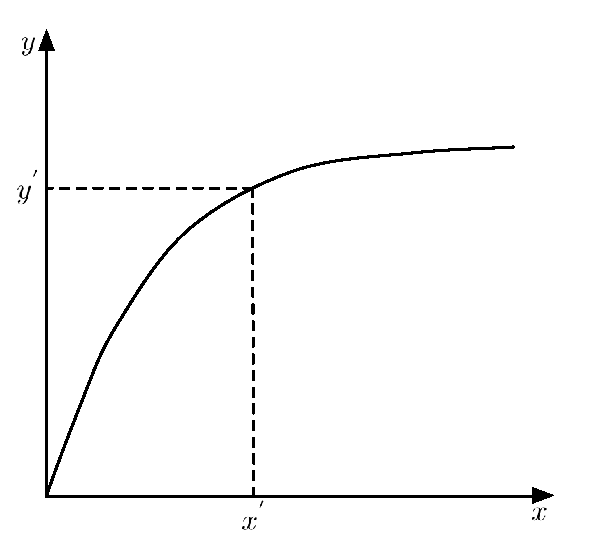
\includegraphics[width=\textwidth]{crisp-f-crisp-xy}
    \caption{Чёткая функция, чёткий аргумент}
  \end{subfigure}
  \quad
  \begin{subfigure}[t]{0.4\textwidth}
    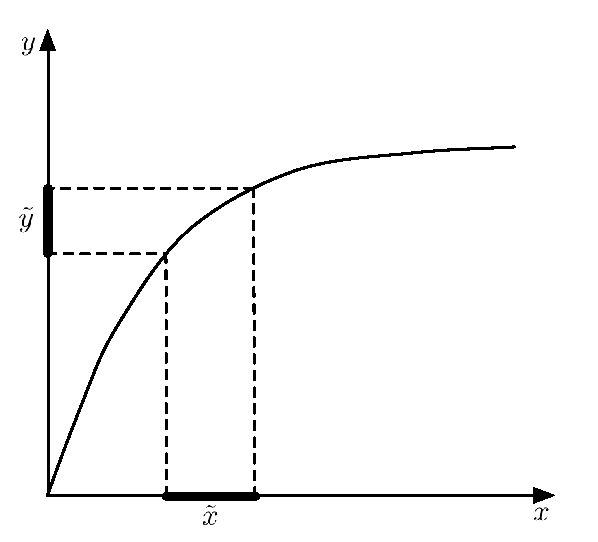
\includegraphics[width=\textwidth]{crisp-f-fuzzy-xy}
    \caption{Чёткая функция, нечёткий/интервальный аргумент}
  \end{subfigure}
  
  \begin{subfigure}[h]{0.4\textwidth}
    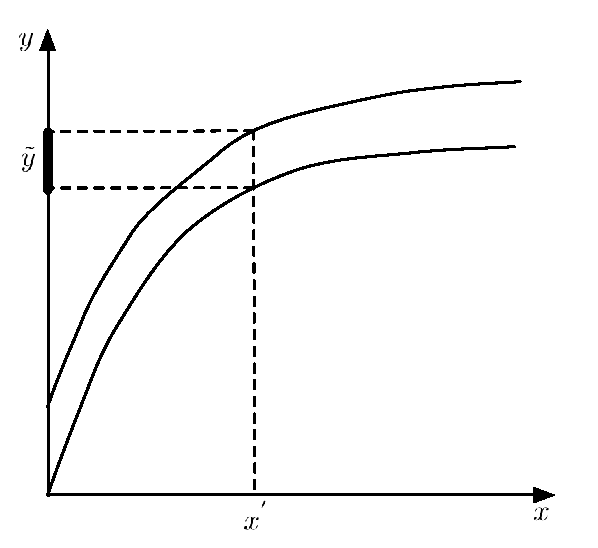
\includegraphics[width=\textwidth]{interval-f-crisp-xy}
    \caption{Интервальная функция, чёткий аргумент}
  \end{subfigure}
  \quad
  \begin{subfigure}[h]{0.4\textwidth}
    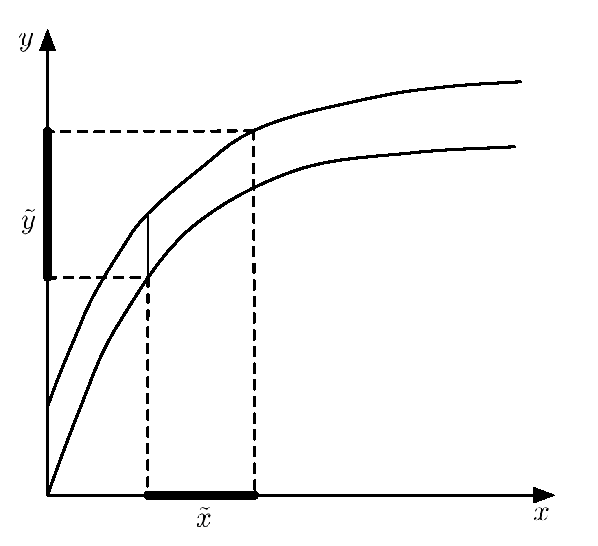
\includegraphics[width=\textwidth]{interval-f-fuzzy-xy}
    \caption{Интервальная функция, интервальный/нечёткий аргумент}
  \end{subfigure}
  
  \begin{subfigure}[b]{0.4\textwidth}
    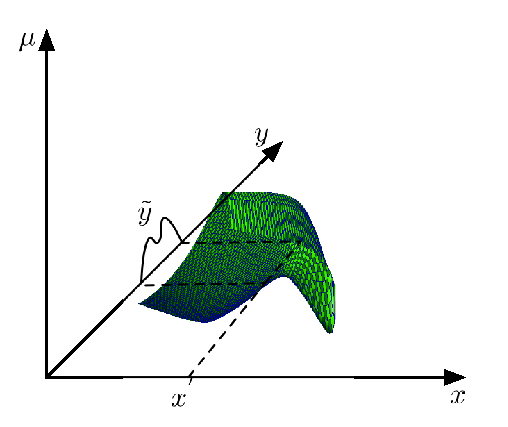
\includegraphics[width=\textwidth]{fuzzy-f-crisp-xy}
    \caption{Нечёткая функция, чёткий аргумент}
  \end{subfigure}
  \quad
  \begin{subfigure}[b]{0.4\textwidth}
    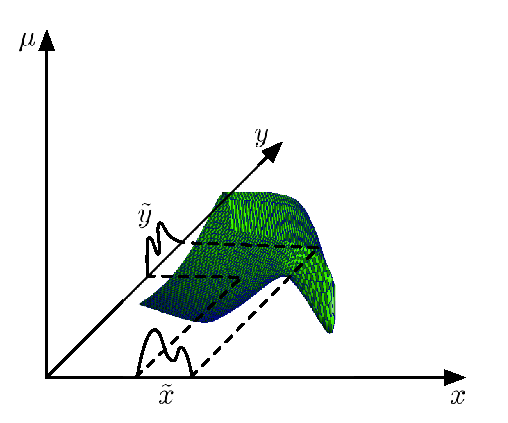
\includegraphics[width=\textwidth]{fuzzy-f-fuzzy-xy}
    \caption{Нечёткая функция, интервальный/нечёткий аргумент}
  \end{subfigure}
  \caption{Результаты вычислений для чётких, интервальных и нечётких функций при чётких и нечётких параметрах}
  \label{fig:functypes-restypes}
\end{figure}

На основании этого примера и категорий неопределённости, выделенных в~\cite{Yarushkina}, можно выделить взаимосвязи между описаниями и переменными чётких и нечётких моделей, а также математические методы, которые применимы для описания моделей. Выделенные взаимосвязи изображены в таблице~\ref{t:fuzzy-modeling-approaches}.
\begin{table}[h!]
\caption{Взаимосвязи между описаниями и переменными чётких и нечётких моделей}
\label{t:fuzzy-modeling-approaches}
\begin{center}
\begin{tabularx}{\textwidth}{|p{0.15\linewidth}|p{0.15\linewidth}|p{0.15\linewidth}|X|}
	\hline
		\centering \textit{Описание модели} & \centering \textit{Входные данные} & \centering \textit{Выходные данные} & \centering \textit{Математические методы} \tabularnewline	\hline
	\hline
		Чёткое & Чёткие & Чёткие & Функциональный анализ, линейная алгебра и т.д. \tabularnewline
	\hline
		Чёткое & Нечёткие & Нечёткие & Принцип обобщения Заде \tabularnewline
	\hline
		Чёткое & Нечёткие & Чёткие & Нечёткие модели и вычисления \tabularnewline
	\hline
		Нечёткое & Чёткие/\allowbreak Нечёткие & Нечёткое & Нечёткие модели и вычисления \tabularnewline
  \hline
\end{tabularx}
\end{center}
\end{table}

Очевидно, что нечёткое моделирование не подменяет собой другие методологии моделирования сложных систем, в которых существенные зависимости выражены настолько хорошо, что они могут быть выражены в числах или символах, получающих в итоге численные оценки~\cite{Borisov_Fedulov}. Нечёткие модели скорее представляют необходимый инструмент для исследования как отдельных аспектов, так и системы в целом на различных этапах её анализа в случае доминирования качественных элементов над количественными. Об этом же говорится и в~\cite{Kaufmann, Borisov_Alexeev_Msk}~--- теория нечётких множеств не призвана конкурировать с теорией вероятности и статистическими методами, она заполняет пробел в области структуризованной неопределённости там, где нельзя корректно применять статистику и вероятности ввиду неизвестности распределения величин или малого размера статистической выборки.

В~\cite{Borisov_Fedulov} предложена оригинальная классификация подходов к созданию нечётких моделей в~зависимости от~того, в~какой момент моделирования используется теория нечётких множеств, а~также соответствующие ей сферы применения нечётких моделей. Рассмотрим данную классификацию подробнее: нечёткость может применяться
\begin{enumerate}
	\item при описании системы~--- речь идёт об информационной неопределённости~\cite{Pospelov, Borisov_Alexeev_Msk}. Система описывается моделями нечёткой логики: продукционными/реляционными/функциональными. Обычно такой подход применяется, когда имеются неполные или неопределённые знания об исследуемом объекте, а их дополнение является либо невозможным, либо нецелесообразным, либо значительная часть информации об объекте является качественной и не~выражается с~помощью известных математических зависимостей, но может быть описана системой предпочтений на~естественном языке в форме правил <<если-то>>;
	\item при задании параметров системы~--- в традиционной, чёткой модели системы используются нечёткие параметры (например, нечёткие коэффициенты обычных алгебраических или дифференциальных уравнений). Данный подход оправдывает себя в ситуации полной определённости модели, когда необходимо учесть присущую параметрам неопределённость, а традиционный вероятностный подход неприменим ввиду того, что неоднозначность параметров не является физической согласно классификации, используемой в~\cite{Borisov_Alexeev_Msk, Yarushkina}. В таких ситуациях приходится прибегать к~услугам экспертов, которые выражают своё мнение в виде качественных оценок, а принадлежность объектов задаётся с помощью лингвистических операторов («много», «мало», «около» и т.п.);
	\item нечёткость при~задании входов, выходов и состояний системы~--- в традиционной модели системы с чёткими или нечёткими параметрами могут применяться нечёткие переменные. Этот подход в основном применяется при идентификации динамических или нелинейных систем на основе их входных и выходных параметров~\cite{Fuller} и позволяет при наличии обучающей выборки аппроксимировать искомые функции или измеренные данные с наперёд заданной точностью;
	\item комбинированные модели~--- создаются на основе совмещения двух или более подходов.
\end{enumerate}

Если рассматривать описанную выше классификацию подходов к синтезу нечётких моделей через призму выбора, который являются неотъемлемой частью моделирования как целенаправленного процесса, и языков его описания, то можно заметить, как модель и используемый в ней язык выбора проецируются на~два основных раздела современной нечёткой математики~--- нечёткий логический вывод и мягкие вычисления. К настоящему моменту сложилось три основных языка описания выбора~--- язык функций выбора, язык бинарных отношений и критериальный язык~\cite{Choice_Languages}, которые позволяют говорить об одном и том же объекте или явлении с разной степенью общности. Два последних языка~--- язык бинарных отношений и критериальный язык~--- достаточно хорошо изучены и отражены в рамках теории нечётких множеств. Схематически взаимосвязи между сферами нечёткого моделирования и~языками выбора изображены на~рисунке~\ref{fig:choice-classes}.

\begin{figure}[t!]
  \centering{
    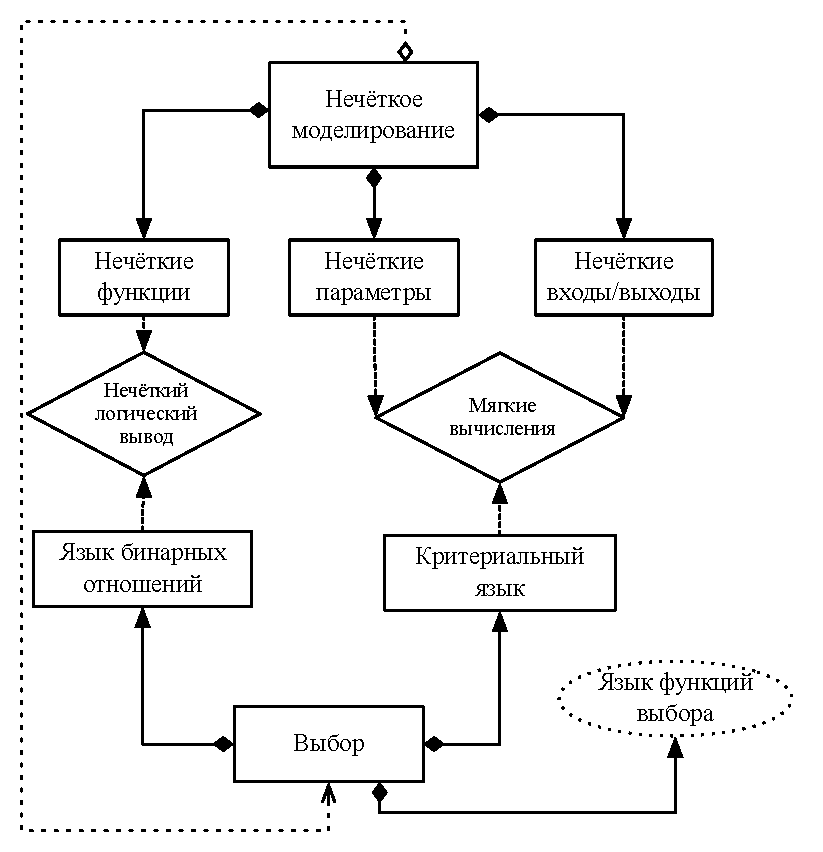
\includegraphics[width=0.7\textwidth]{choice-classification}
    \caption{Связь между языками описания выбора и нечётким моделированием}
    \label{fig:choice-classes}
  }
\end{figure}

Язык бинарных отношений является более общим и основывается на том факте, что в~реальности дать объективную оценку той или~иной альтернативе затруднительно или невозможно, однако, при~рассмотрении альтернатив в~паре, можно указать более или~менее предпочтительную. Основные предположения этого~языка выбора сводятся к~следующим:
\begin{itemize}
	\item отдельная альтернатива не~оценивается;
	\item для~каждой пары альтернатив некоторым образом можно установить, что~одна из~них предпочтительнее другой, либо они равноценны или несравнимы;
	\item отношение предпочтения внутри любой пары альтернатив не~зависит от~остальных альтернатив, предъявленных к~выбору.
\end{itemize}

Нечёткие модели первого типа, в которых нечёткость присутствует на этапе описания системы~\cite{Choice_Languages}, как раз используют язык бинарных отношений. В~нечёткой математике этот язык проецируется на нечёткий логический вывод и основанное на нём нечёткое управление. Основополагающими для логического вывода являются понятия нечёткого отношения, лингвистической переменной и нечёткой импликации, на которой основаны правила логического вывода.

\begin{mydef}
Лингвистической переменной называется переменная, значения которой представляют слова или суждения на естественном языке. С точки зрения нечёткой математики, это кортеж $\left\lbrace \beta, T, X, G, M \right\rbrace$, где $\beta$~--- название нечёткой переменной; $T$~--- базовое терм-множество лингвистической переменной, каждый элемент которого (терм) представляется как нечеткое множество на универсальном множестве $X$; $G$~--- cинтаксические правила, часто задаваемые в виде грамматики, для порождения названий термов; $M$~--- семантические правила, задающие функции принадлежности нечетких термов, порожденных синтаксическими правилами $G$ \cite{Uskov_Kuzmin, Uskov_Kruglov, Shtovba}.
\end{mydef}

\begin{mydef}
Нечёткая импликация является нечётким отношением $\tilde R \subseteq X \times Y$, простейшая форма которого выражается в~виде правила <<если-то>>~\cite{Pegat}
\begin{equation}
  IF \left( x = \tilde A \right) THEN \left( y = \tilde B\right),\ x \in X, y \in Y.
\end{equation}
Нечёткая импликация обозначается как $\tilde A \rightarrow \tilde B$ и, как любое другое нечёткое отношение, задаётся функцией принадлежности.
\end{mydef}
В~\cite{Pegat, Rutkovskaya} описаны несколько применяемых на практике операторов импликации, задаваемых различными функциями принадлежности (например, операторы Мамдани, Лукасевича, Ларсена, Гёделя, Ягера, Заде).

На основании нечётких переменных и правил импликации строятся модели нечёткого логического вывода и управления. Типовая модель включает в~себя четыре основных блока~\cite{Fuller}, изображённые на рисунке~\ref{fig:general-fuzzy-inference}~--- блок фаззификации, который сопоставляет чётким входным значениям нечёткие множества; блок нечёткого логического вывода, опирающийся на базу правил, хранящуюся в виде нечётких импликаций <<если-то>>; блок дефаззификации, который на основании результирующей функции принадлежности формирует чёткое выходное значение с помощью одного из методов дефаззификации (центра тяжести, первого/среднего/последнего максимума, центра сумм и др.)~\cite{Pegat, Uskov_Kuzmin, Uskov_Kruglov, Zak}. Наиболее популярными моделями являются нечёткие контроллеры Такаги-Сугено и~Мамдани, применяемые, в частности, в~качестве нечётких регуляторов в~промышленной и~бытовой электронике~\cite{Grinyaev_Computerra}.

\begin{figure}[h!]
  \centering{
    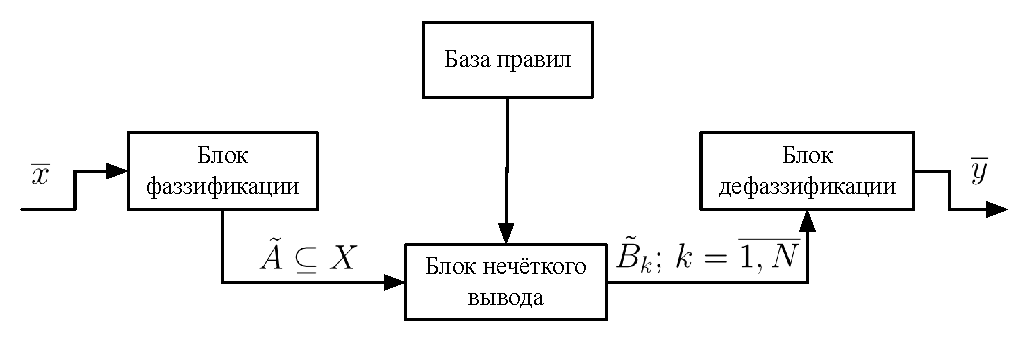
\includegraphics[width=\textwidth]{fuzzy-inference}
    \caption{Общая схема системы нечёткого управления}
    \label{fig:general-fuzzy-inference}
  }
\end{figure}

Достоинства и недостатки, а также рекомендации по применению нечёткого логического вывода и нечёткого управления хорошо описаны в~\cite{Bauer_Winkler, Grinyaev_Computerra}. Согласно~\cite{Bauer_Winkler, Pavlov_Sokolov}, использование моделей первого типа рекомендуется для моделирования очень сложных процессов, когда не существует простой математической модели, для нелинейных процессов высоких порядков и для~обработки лингвистически сформулированных экспертных знаний. Ещё одним преимуществом является наличие нескольких подходов к проверке моделей на устойчивость~\cite{Pegat, Uskov_Kruglov}. Эти же модели не рекомендуется применять, если приемлемый результат может быть получен с~помощью общей теории управления, либо существует формализованная и адекватная математическая модель, либо проблема не разрешима методами современной математики. Также модели нечёткого управления страдают от~<<проклятия размерности>>~--- с увеличением числа входов лавинообразно нарастает число необходимых правил для вывода~\cite{Pegat, Fuller}. Нечёткому логическому выводу и~управлению посвящено множество книг и~публикаций, однако подробное рассмотрение моделей первого вида выходит за~рамки данной диссертации.

Второй язык, более простой и~узкий, однако и~более изученный~--- критериальный. Он~основывается на~предположении, что~каждую отдельно взятую альтернативу возможно оценить конкретным числом, называемым значением критерия. Сравнение альтернатив в~таком случае сводится к~сравнению соответствующих~им числовых значений. Пусть $x\in X$ - некоторая альтернатива из~множества альтернатив $X$. Критерием будем называть функцию $q\left( x \right),\ x\in X$, обладающую тем~свойством, что~если альтернатива ${x_1}$ предпочтительнее ${x_2}$, то $q\left( x_1 \right)>q\left( x_2 \right)$ и~наоборот. Естественно считать, что наилучшей альтернативой ${{x}^{*}}$ считается~та, значение критерия которой максимально:
\begin{equation*}
  x^{*}=\arg \underset{i}{\mathop{\max }}\,\left\{ q\left( x_i \right) \right\}
\end{equation*}
Задача отыскания $x^{*}$, достаточно простая по~постановке, часто оказывается весьма сложной в решении, поскольку зависит от характера множества $X$ и критерия $q\left( x \right)$. 

Нечёткие модели второго и третьего типа, в которых нечёткими являются либо их параметры, либо состояния и входные и выходные данные, описываются с помощью критериального языка. Этот язык в~нечёткой~математике соответствует т.\,н. <<мягким вычислениям>>~--- нечётким множествам, нечётким числам и определённым на них алгебрам. Как уже упоминалось ранее, описание с помощью нечётких множеств имеет существенные преимущества перед языком теории вероятностей в том случае, когда имеется лингвистическая неоднозначность в смысле полисемии~\cite{Borisov_Alexeev_Msk}, и~оценки получаются c помощью опроса экспертов. Известно, что люди в большинстве своём неправильно оценивают вероятности (особенно большие и малые), поэтому требовать от экспертов, коими обычно являются специалисты в конкретных предметных областях, а не математики, оценок в форме распределения вероятностей зачастую невозможно~\cite{Gubko}. Кроме того, описание в форме нечётких множеств гораздо менее требовательно к квалификации экспертов и зачастую гораздо точнее отражает суть исследуемого объекта или явления~\cite{Fuller}.

Данная диссертация посвящена исследованию способов представления нечёткости в моделях второго типа, в которых отношения и функции чёткие, а параметры заданы нечёткими числами. Требования, выдвигаемые к алгебраическим структурам над множеством нечётких чисел, которые применяются в~нечётких моделях второго типа, изложены в следующем параграфе.

\section{Возможные направления достижения требований к численной реализации решений} 
\label{chapter1_3}
Понятие алгебраической системы как совокупности алгебры и модели.
 
Необходимым условием четкого равенства должно быть наличие групповых свойств операций над нечеткими числами. Т.е. надо подобрать такую модель представления нечеткой числовой информации, которая при сохранении основных исходных свойств экспертных оценок обеспечивает возможность построения алгебры нечетких чисел эквивалентной  полю действительных чисел. Это обеспечит ограничение роста неопределенности.

Полный порядок должен обеспечиваться выбором подходящей модели в рамках соответствующей алгебраической системы.

Надо выбрать такие условия устойчивости, которые можно было бы использовать непосредственно в алгоритме решения. Более того, модель представления нечеткой числовой информации должна позволять управлять устойчивостью

\subsection{Общие алгебраические структуры}

Для~решения задач с использованием нечётких параметров необходимо уметь выполнять различные операции над нечёткими числами. В различных работах вводятся различные алгебры нечётких чисел. Однако для начала рассмотрим, как вводится понятие алгебры и как оно проецируется на множество нечётких чисел.

Предметом рассмотрения абстрактной алгебры являются произвольные множества с~заданными на~них операциями, при этом природа этих~множеств и~операций может существенно отличаться от~привычных числовых множеств и~известных операций над~числами \cite{Bauman_DM}. Проблема работы со~сложно организованными числовыми и~нечисловыми структурами возникла в~связи с~развитием современных информационных технологий и~переходом от~обычных вычислений к~обработке сложных структур данных.

\begin{mydef}
Пусть $A$ – произвольное непустое множество, $n\in \mathbb{N}$. Любое отображение 
\[
	f:A^N \to A
\] 
называют $n$-арной операцией на множестве $A$.
\end{mydef}

В алгебрах наиболее важными и исследуемыми являются бинарные $\left( n=2 \right)$ операции. Если $*$~--- некая абстрактная бинарная операция, то, согласно \cite{Bauman_DM}, она~является
\begin{itemize}
	\item коммутативной, если $\forall x,y\in A\ x*y=y*x$;
	\item ассоциативной, если $\forall x,y,z\in A\ x*\left( y*z \right)=\left( x*y \right)*z$;
	\item идемпотентной, если $\forall x\in A\ x*x=x$.
\end{itemize}

Элемент $0$ множества $A$ называют нулём относительно операции $*$, если $\forall x\in A\ 0*x=0,\ x*0=0$. Нуль в множестве $A$ единственен. В~самом деле, если~предположить существование другого нулевого элемента ${0}'$ относительно операции $*$, то,~согласно определению нуля
\[
	0*{0}'=0,\ {0}'*0={0}'
\],
откуда следует равенство $0={0}'$.

Элемент 1 множества $A$ называют нейтральным относительно операции $*$, если $\forall x\in A\ 1*x=x,\ x*1=1$.
Нейтральный элемент в множестве $A$ также единственен, доказательство этого факта аналогично доказательству единственности нулевого элемента.

В~\cite{Bauman_DM, Adelson_Velskiy} даётся следующее определение алгебры.
\begin{mydef}
Алгебра считается заданной, если задано некоторое множество $D$, называемое носителем алгебры, и некоторое множество операций $\Omega $ на $D$, называемое сигнатурой данной алгебры. Алгебру можно записать как упорядоченную пару множеств $\left( D,\Omega  \right)$.
\end{mydef}

Стоит отметить, что~операции, включенные в~сигнатуру, задаются как~некоторые специальные отображения. При~этом не~оговариваются свойства, которыми операции обладают на~носителе~--– они обычно указываются дополнительно.
Кратко рассмотрим основные виды алгебр, описанные в~\cite{Bauman_DM, Adelson_Velskiy, Voevodin},. Вначале дадим определения для алгебр, сигнатура которых состоит из одной абстрактной бинарной операции $*$.

Группоидом называют любую алгебру $\left( D,* \right)$, сигнатура которой состоит из~одной бинарной операции, на~которую не~наложено никаких ограничений. Если~же операция $*$ ассоциативна, то~группоид является полугруппой. Отдельно выделяют коммутативные полугруппы~--– полугруппы, в~которых операция $*$ обладает свойством коммутативности.

Моноидом называется такая полугруппа, относительно операции которой существует нейтральный элемент. Такой элемент называется единицей моноида $\left( D,* \right)$ и~обозначается как 1. Для моноида справедливы следующие свойства:
\begin{itemize}
	\item $\forall x,y,z\in D\quad x*\left( y*z \right)=\left( x*y \right)*z$;
	\item $\forall x\in D\quad x*1=1*x=x$.
\end{itemize}

Если в моноиде $\forall x\in D\ \exists \,{{x}^{-1}}\in D$, называемый обратным, такой, что~$x*{{x}^{-1}}={{x}^{-1}}*x=1$, то~моноид является группой. В~\cite{Bauman_DM, Adelson_Velskiy, Voevodin} доказывается теорема о~единственности обратного элемента для~каждого~$x\in D$. Если~же операция~$*$ коммутативна, то~группа называется абелевой. Для~абелевой~группы свойства моноида дополняются ещё двумя~свойствами:
\begin{itemize}
	\item $\forall x,y\in D\quad x*y=y*x$;
	\item $\forall x\in D\quad x*{{x}^{-1}}=1$.
\end{itemize}

Для~наглядности записи, в~сигнатуру алгебры допускается включать нейтральные относительно операции элементы, поскольку, как указано в [21-томник], они являются нульарной операцией. В этом случае моноид можно записать как совокупность $\left( D,*,1 \right)$.

Перейдём к рассмотрению алгебр с сигнатурой, состоящей из двух бинарных операций. Кольцом называют алгебру $\left( D,+,\cdot ,1,0 \right)$, такую, что алгебра $\left( D,+,0 \right)$ является абелевой группой, алгебра $\left( D,\cdot ,1 \right)$ является моноидом, а операция умножения кольца $\left( \cdot  \right)$ дистрибутивна относительно операции сложения кольца $\left( + \right)$, т.е. справедливо равенство:
	\[\forall x,y,z\in D:\quad x\cdot \left( y+z \right)=x\cdot y+x\cdot z\].
Элементы 0~и~1 называют нулём и~единицей кольца соответственно. Если операция~умножения коммутативна, то~кольцо является коммутативным.

Если~же в~кольце алгебра всех ненулевых по~умножению элементов кольца образует группу, то~кольцо называется телом. Коммутативное же~тело является полем. Другими словами, поле есть алгебра $\left( D,+,\cdot ,0,1 \right)$, сигнатура которой состоит из~двух бинарных и~двух нульарных операций, для~которых должны выполняться следующие тождества \cite{Adelson_Velskiy, Bauman_DM, Yakhyaeva}:
\begin{enumerate}
	\item ассоциативность по сложению: $\forall x,y,z\in D:\ x+\left( y+z \right)=\left( x+y \right)+z$;
	\item коммутативность по сложению: $\forall x,y\in D:\ x+y=y+x$;
	\item наличие нуля (нейтрального по сложению элемента): $\exists \,0\in D:\ \forall x\in D\ \ x+0=x$;
	\item существование противоположного элемента:$\forall x\in D\ \exists \,-x\in D:\ x+\left( -x \right)=0$;
	\item ассоциативность по умножению: $\forall x,y,z\in D:\ x\cdot \left( y\cdot z \right)=\left( x\cdot y \right)\cdot z$;
	\item коммутативность по умножению: $\forall x,y\in D:\ x\cdot y=y\cdot x$;
	\item наличие единицы (нейтрального по умножению элемента): $\exists \,1:\ \forall x\in D:\ x\cdot 1=x$;
	\item существование обратного элемента для ненулевых элементов: $\forall x\in D\backslash \left\{ 0 \right\}\ \ \exists \ {{x}^{-1}}:\ \ x\cdot {{x}^{-1}}=1$;
	\item дистрибутивность умножения относительно сложения: $\forall x,y,z\in D:x\cdot y+x\cdot z=x\cdot \left( y+z \right)$.
\end{enumerate}

\subsection{Анализ существующих алгебр нечётких чисел}

В~чётких задачах в~качестве параметров используются элементы множества действительных чисел $\mathbb{R}$, на~котором определена алгебра действительных чисел, являющаяся по~своей структуре полем. Для~того, чтобы нечёткие числа можно было применять в~качестве параметров чётких задач, алгебра, применяемая к~ним, также должна быть полем.

%В~отечественной и~зарубежной литературе вводится множество различных алгебр нечётких чисел, однако концептуально они различаются только по тому, используется ли в них принцип обобщения Заде (обычный или~$\alpha$-уровневый) или~нет. Также существующие алгебры нечётких чисел можно классифицировать с точки зрения свойств их операций (моноиды, группоиды, кольца и т.д.).

\subsubsection*{Вычисления с использованием интервальной нечёткости}
Как указано в~\cite{Rotshtein, Borisov_Krumberg_Riga}, алгебры, основанные на~принципе~обобщения Заде, обладают существенным недостатком~--- неэффективными промежуточными вычислениями, необходимыми для получения функции принадлежности результата. Поскольку для~нечётких~множеств справедлива теорема о декомпозиции, то для решения практических задач, обычная нечёткость может быть сведена к интервальной, а операции над числами – к соответствующим операциям над их $\alpha$-сечениями. В~\cite{Borisov_Krumberg_Riga} предлагается выполнить дискретизацию непрерывного нечёткого числа по конечному числу $\alpha$-уровней $\alpha_i;i=\overline{1,k}$, причём $\alpha_1=0$, $\alpha_k=1$. Нечёткое число будет представлено совокупностью интервалов $\displaystyle \bigcup\limits_{i=1}^{k}{{{\left[ {{x}_{i1}};{{x}_{i2}} \right]}_{{{\alpha }_{i}}}}}$, над которыми можно совершать некоторые операции.

В~статье~\cite{Levin} описывается алгебра для~интервалов вида $\tilde{x}=\left[ {{x}_{1}};{{x}_{2}} \right];\,{{x}_{1}}\le {{x}_{2}};\ {{x}_{1}},{{x}_{2}}\in \mathbb{R};\ \ \tilde{x}\in X$. Произвольная интервальная функция $F\left( \tilde{x},\tilde{y},...,\tilde{z} \right)$ определяется с помощью сопоставленной ей чёткой функции $f\left( x,y,...,z \right)$, $x\in \tilde{x}$, $y\in \tilde{y}$, …$z\in \tilde{z}$ следующим образом:
\begin{equation}
\label{eq:interval-function}
	F\left( \tilde{x},\tilde{y},...,\tilde{z} \right)=\left\{ f\left( x,y,...,z \right)\left| x\in \tilde{x},y\in \tilde{y},...,z\in \tilde{z} \right. \right\}
\end{equation}

В~соответствие с~определением~\eqref{eq:interval-function}, автор вводит конкретные алгебраические операции для интервалов:
\begin{itemize}
	\item сложение $\tilde{v}=\tilde{x}+\tilde{y}=\left\{ \left( x+y \right)\left| x\in \tilde{x},y\in \tilde{y} \right. \right\}=\left[ {{x}_{1}}+{{y}_{1}};{{x}_{2}}+{{y}_{2}} \right]$;
	\item вычитание $\tilde{v}=\tilde{x}-\tilde{y}=\left\{ \left( x-y \right)\left| x\in \tilde{x},y\in \tilde{y} \right. \right\}=\left[ {{x}_{1}}-{{y}_{2}};{{x}_{2}}-{{y}_{1}} \right]$;
	\item умножение на число: $\tilde{v}=k\tilde{x}=\left\{ kx\left| x\in \tilde{x},k\in \mathbb{R} \right. \right\}=\left[\underset{i}{\mathop {\min}} \left( kx_i \right); \underset{i}{\mathop {\max}} \left( kx_i \right) \right]$;
	
%	\left\{ \begin{aligned}
% & \left[ k{{x}_{1}};k{{x}_{2}} \right];k\geqslant 0 \\ 
%& \left[ k{{x}_{2}};k{{x}_{1}} \right];k<0 \\ 
%\end{aligned} \right.$;
	\item умножение $\tilde{v}=\tilde{x}\cdot \tilde{y}=\left\{ \left( x\cdot y \right)\left| x\in \tilde{x},y\in \tilde{y} \right. \right\}=\left[ \underset{i,j}{\mathop{\min }}\,\left( {{x}_{i}}{{y}_{j}} \right);\underset{i,j}{\mathop{\max }}\,\left( {{x}_{i}}{{y}_{j}} \right) \right]$;
	\item деление $\displaystyle \tilde{v}=\frac{{\tilde{x}}}{{\tilde{y}}}=\left\{ \left. \left( \frac{x}{y} \right) \right|x\in \tilde{x},y\in \tilde{y} \right\}=\left[ {{x}_{1}};{{x}_{2}} \right]\cdot \left[ \frac{1}{{{y}_{2}}};\frac{1}{{{y}_{1}}} \right]$.
\end{itemize}

Также определяются интервальная единица $\tilde{1}=\left[ 1;1 \right]$ и интервальный ноль $\tilde{0}=\left[ 0;0 \right]$ как нейтральные элементы по умножению и сложению соответственно. Во вводимой алгебре справедливы следующие законы:
\begin{enumerate}
	\item коммутативность по сложению $\tilde{x}+\tilde{y}=\tilde{y}+\tilde{x};\ \ \tilde{x},\tilde{y}\in X$;
	\item ассоциативность по сложению $\tilde{x}+\left( \tilde{y}+\tilde{z} \right)=\left( \tilde{x}+\tilde{y} \right)+\tilde{z};\ \tilde{x},\tilde{y},\tilde{z}\in X$;
	\item коммутативность по умножению $\tilde{x}\cdot \tilde{y}=\tilde{y}\cdot \tilde{x};\ \ \tilde{x},\tilde{y}\in X$;
	\item ассоциативность по умножению $\tilde{x}\cdot \left( \tilde{y}\cdot \tilde{z} \right)=\left( \tilde{x}\cdot \tilde{y} \right)\cdot \tilde{z};\ \ \tilde{x},\tilde{y},\tilde{z}\in X$;
	\item существование единственного нейтрального по сложению элемента (нуля) $\tilde{x}+\tilde{0}=\tilde{0}+\tilde{x}=\tilde{x};\ \tilde{x}\in X$;
	\item существование единственного нейтрального по умножению элемента (единицы) $\tilde{x}\cdot \tilde{1}=\tilde{1}\cdot \tilde{x}=\tilde{x};\ \tilde{x}\in X$;
	\item дистрибутивность умножения на действительную константу относительно сложения $k\left( \tilde{x}+\tilde{y} \right)=k\tilde{x}+k\tilde{y};\ \ \tilde{x},\tilde{y}\in X,\ k\in \mathbb{R}$.
\end{enumerate}

Как~отмечается в~\cite{Pospelov, Sokolov}, интервальная алгебра определяет операции вычитания и~деления как самостоятельные операции, при~этом, в~общем~случае, интервальные числа не обладают свойством дистрибутивности умножения относительно сложения; отсутствуют понятия противоположного элемента (по сложению) и обратного элемента (по умножению); вычитание из~интервального числа равного ему в~общем~случае не~приводит к~нуль-интервалу, как и деление интервального числа на равное ему не дает вырожденного единичного интервала. Эти недостатки подтверждаются в~\cite{Levin} в~виде следующих законов:
\begin{enumerate}
	\item $\tilde{x}-\tilde{x}=\tilde{0}\Leftrightarrow \tilde{x}=\left[ {{x}_{1}};{{x}_{1}} \right]$, т.е. разность интервального числа самого с собой равна нулю тогда и только тогда, когда это число вырожденное;
	\item $\displaystyle \frac{{\tilde{x}}}{{\tilde{x}}}=\tilde{1}\Leftrightarrow \tilde{x}=\left[ {{x}_{1}};{{x}_{1}} \right]$, т.е. результат деления интервального числа на само себя равен единице в том и только в том случае, когда это число вырожденное;
	\item противоположные по сложению элементы существуют только для вырожденных интервалов: $\tilde{x}+\tilde{y}=\tilde{0}\Leftrightarrow \tilde{x}=\left[ {{x}_{1}};{{x}_{1}} \right];\tilde{y}=\left[ -{{{\tilde{x}}}_{1}};-{{{\tilde{x}}}_{1}} \right]$;
	\item обратные по умножению элементы существую только для вырожденных интервалов: $\displaystyle \tilde{x}\cdot \tilde{y}=\tilde{1}\Leftrightarrow \tilde{x}=\left[ {{x}_{1}};{{x}_{1}} \right];\tilde{y}=\left[ \frac{1}{{{x}_{1}}};\frac{1}{x_1} \right]$;
	\item закон субдистрибутивности умножения на интервальное число относительно сложения $\tilde{x}\cdot \left( \tilde{y}+\tilde{z} \right)\subseteq \tilde{x}\cdot \tilde{y}+\tilde{x}\cdot \tilde{z}$. Только в частном случае, когда $\tilde y,\tilde z>\tilde 0$, имеет место истинная дистрибутивность.
\end{enumerate}

Как указано в~\cite{Levin}, невыполнение некоторых аксиом поля, а также перечисленные выше особенности интервальных чисел приводят к значительной специфике их использования на практике (в основном, для оценки множества решений некоторой задачи при интервально заданных параметрах). Стоит также упомянуть описанную в~\cite{Spesivtsev, Yakhyaeva} проблему размытости произведения, т.\,е. необоснованного увеличения нечёткости. Размытость зависит не только от длины $d={{x}_{2}}-{{x}_{1}}$ интервала, но и от его положения на~числовой~оси. К~примеру, интервалы одинаковой длины $\left[ 1;3 \right]$ и $\left[ 99;101 \right]$, будучи умноженными на один и тот же интервал$\left[ 2;4 \right]$, дадут результаты с сильно различающейся степенью нечёткости:
\[
	\begin{matrix}
		\left[ 2;4 \right]\cdot \left[ 1;3 \right]=\left[ 2;12 \right];\quad d=12-2=10 \\ 
		\left[ 2;4 \right]\cdot \left[ 99;101 \right]=\left[ 198;404 \right];\quad d=404-198=206 
	\end{matrix}
\]

\subsubsection*{Алгебры нечётких LR-чисел}

% (Поспелов + [28], Борисов + [54] [107] [25])
На практике для нечётких вычислений часто используются удобные для понимания и записи нечёткие числа $LR$-типа. Такое число, согласно определению, представимо в виде тройки $\tilde{A}=\left( m;a;b \right)$. Арифметические операции над~числами $LR$-типа в~\cite{Pospelov, Yakhyaeva} вводятся следующим образом:
\begin{itemize}
	\item сложение ${{\tilde{A}}_{1}}+{{\tilde{A}}_{2}}$ : $\left( {{m}_{1}},{{a}_{1}},{{b}_{1}} \right)+\left( {{m}_{2}},{{a}_{2}},{{b}_{2}} \right)=\left( {{m}_{1}}+{{m}_{2}},{{a}_{1}}+{{a}_{2}},{{b}_{1}}+{{b}_{2}} \right)$;
	\item противоположное число $-{{\tilde{A}}_{1}}$: $-\left( m,a,b \right)=\left( -m,b,a \right)$;
	\item вычитание вводится как сумма числа ${{\tilde{A}}_{1}}$ и~числа, противоположного числу ${{\tilde{A}}_{2}}$: $\left( {{m}_{1}},{{a}_{1}},{{b}_{1}} \right)-\left( {{m}_{2}},{{a}_{2}},{{b}_{2}} \right)=\left( {{m}_{1}}-{{m}_{2}},{{a}_{1}}+{{b}_{2}},{{b}_{1}}+{{a}_{2}} \right)$;
	\item умножение положительных чисел: $\left( {{m}_{1}},{{a}_{1}},{{b}_{1}} \right)\times \left( {{m}_{2}},{{a}_{2}},{{b}_{2}} \right)=\left( {{m}_{1}}{{m}_{2}},{{m}_{2}}{{a}_{1}}+{{m}_{1}}{{a}_{2}},{{m}_{2}}{{b}_{1}}+{{m}_{1}}{{b}_{2}} \right)$;
	\item умножение разнознаковых чисел $\left( {{m}_{1}},{{a}_{1}},{{b}_{1}} \right)\times \left( {{m}_{2}},{{a}_{2}},{{b}_{2}} \right)=\left( {{m}_{1}}{{m}_{2}},{{m}_{2}}{{a}_{1}}-{{m}_{1}}{{b}_{2}},{{m}_{2}}{{b}_{1}}-{{m}_{1}}{{a}_{2}} \right)$;
	\item умножение отрицательных чисел $\left( {{m}_{1}},{{a}_{1}},{{b}_{1}} \right)\times \left( {{m}_{2}},{{a}_{2}},{{b}_{2}} \right)=\left( {{m}_{1}}{{m}_{2}},-{{m}_{2}}{{b}_{1}}-{{m}_{1}}{{b}_{2}},-{{m}_{2}}{{a}_{1}}-{{m}_{1}}{{a}_{2}} \right)$;
	\item обратное число $\displaystyle {\tilde A}^{-1}$: ${{\left( m,a,b \right)}^{-1}}=\left( \frac{1}{m};\frac{b}{{{m}^{2}}};\frac{a}{{{m}^{2}}} \right)$;
	\item деление нечётких чисел $\displaystyle \frac{{{{\tilde{A}}}_{1}}}{{{{\tilde{A}}}_{2}}}$ рассматривается~как умножение числа ${{\tilde{A}}_{1}}$ на~число, обратное числу ${{\tilde{A}}_{2}}$: $\displaystyle \left( \frac{{{m}_{1}}}{{{m}_{2}}},\frac{{{m}_{1}}{{b}_{2}}+{{m}_{2}}{{a}_{1}}}{m_{2}^{2}},\frac{{{m}_{1}}{{a}_{2}}+{{m}_{2}}{{b}_{1}}}{m_{2}^{2}} \right)$.
\end{itemize}

Для~вводимых~операций справедливы свойства коммутативности и~ассоциативности операций сложения и~вычитания. Свойство дистрибутивности, как и~в~случае вычислений, основанных~на принципе~Заде, выполняется не~всегда. Кроме того, и~для~этой алгебры нечётких чисел характерны недостатки, описанные в~\cite{Spesivtsev, Yakhyaeva}~--– носитель результата может необоснованно расшириться ввиду зависимости результата от~степени нечёткости операндов и~их~местоположения на~числовой~оси. Также при построении данной алгебры не вводятся нейтральные по сложению и умножению элементы (ноль и единица). В~статье~\cite{Uskov_PPS} отмечается, что~если в~качестве нулевого~элемента использовать тройку, соответствующую нулю во множестве действительных чисел
\begin{equation}
\label{eq:zero-element}
	\tilde{0}=\left( 0;0;0 \right)
\end{equation}
а в~качестве единицы~--– тройку
\begin{equation}
\label{eq:one-element}
	\tilde{1}=\left( 1;0;0 \right)
\end{equation}
то в~этом~случае вводимые ранее операции не~позволяют получить поле из-за~невыполнения тождеств $\tilde{A}+\left( -\tilde{A} \right)=\tilde{0}$ и $\tilde{A}\cdot {{\tilde{A}}^{-1}}=\tilde{1}$.

Для~получения алгебры типа~поле с~использованием нейтральных элементов \eqref{eq:zero-element}~и~\eqref{eq:one-element}, авторы~\cite{Uskov_PPS} предлагают ввести групповые операции над нечёткими числами. Для этого вводятся несколько иные противоположный и~обратный элементы:
\begin{gather}
	\label{eq:reverse-minus-element}
	-\left( m;a;b \right)=\left( -m;-a;-b \right); \\ 
	\label{eq:reverse-div-element}
	\left( m;a;b \right)^{-1}=\left( \frac{1}{m};-\frac{a}{{{m}^{2}}};-\frac{b}{{{m}^{2}}} \right). 
\end{gather}

При~этом признаётся тот~факт, что~вводимые с~помощью~  элементы имеют отрицательные коэффициенты нечёткости, а, следовательно, лишены физического смысла и не являются элементами множества нечётких $LR$-чисел. Однако, согласно определениям, которые вводились при рассмотрении абстрактных алгебр, противоположный и обратный элемент также должны являться элементами несущего множества алгебры, что в (1.35) не выполняется. Таким образом, алгебру групповых нечётких чисел нельзя называть полем в строгом смысле этого термина. Более того, авторы статьи ограничивают применимость вводимой ими алгебры только тем случаем, когда в рассматриваемой задаче есть только один независимый нечёткий параметр/сигнал, поскольку в этом случае предотвращается необоснованное увеличение степени нечёткости результата. Во всех остальных случаях предлагается использовать классический подход к нечётким вычислениям, который был описан выше, со всеми свойственными ему недостатками.
В~статье~\cite{Piter_SCM} на~основании идей, изложенных в~\cite{Borisov_Krumberg_Riga, Alexeev_Riga}, для~решения проблем чрезмерной размытости результата и~нетождественности выражений вида $\tilde A+\tilde B-\tilde B=\tilde A$, вводятся дополнительные арифметические операции и~новое представление нечёткого числа, нечувствительное к~его~знаку. Дополнительной арифметической операцией $\underset{d}{\mathop{*}}\,$ для~операции $*$ является такая, что~для~нечётких чисел $\tilde A. \tilde B, \tilde C$
\begin{equation}
\label{eq:complementary-operations}
	\tilde{C}=\tilde{A}\underset{d}{\mathop{*}}\,\tilde{B}\to \tilde{C}*\tilde{B}=\tilde{A}
\end{equation}

Для определения нового представления нечёткого числа $\left( m,d\left( {\tilde{A}} \right),\Delta \left( {\tilde{A}} \right) \right)$, называемого симметризованным параметрическим, авторы~\cite{Piter_SCM} вводят понятия показателя нечёткости числа $\displaystyle d\left( {\tilde{A}} \right)=\frac{a+b}{2}$ и коэффициента асимметрии $\displaystyle \Delta \left( {\tilde{A}} \right)=\frac{b-a}{2}$. Дополнительные арифметические операции над нечёткими числами в новом представлении выглядят следующим образом:
\begin{gather*}
		\tilde{A}\underset{d}{\mathop{+}}\,\tilde{B}=\left( {{m}_{{\tilde{A}}}}+{{m}_{{\tilde{B}}}};\left| d\left( {\tilde{A}} \right)-d\left( {\tilde{B}} \right) \right|;\Delta \left( {\tilde{A}} \right)+\Delta \left( {\tilde{B}} \right) \right); \\ 
		\tilde{A}\underset{d}{\mathop{-}}\,\tilde{B}=\left( {{m}_{{\tilde{A}}}}-{{m}_{{\tilde{B}}}};\left| d\left( {\tilde{A}} \right)-d\left( {\tilde{B}} \right) \right|;\Delta \left( {\tilde{A}} \right)-\Delta \left( {\tilde{B}} \right) \right); \\ 
		\tilde{A}\underset{d}{\mathop{\cdot }}\,\tilde{B}=\left( {{m}_{{\tilde{A}}}}{{m}_{{\tilde{B}}}};\left| \left| {{m}_{{\tilde{B}}}} \right|d\left( {\tilde{A}} \right)-\left| {{m}_{{\tilde{A}}}} \right|d\left( {\tilde{B}} \right) \right|;\left| {{m}_{{\tilde{A}}}} \right|\Delta \left( {\tilde{B}} \right)+\left| {{m}_{{\tilde{B}}}} \right|\Delta \left( {\tilde{A}} \right) \right); \\ 
		\tilde{A}\underset{d}{\mathop{:}}\,\tilde{B}=\left( \frac{{{m}_{{\tilde{A}}}}}{{{m}_{{\tilde{B}}}}};\frac{\left| \left| {{m}_{{\tilde{B}}}} \right|d\left( {\tilde{A}} \right)-\left| {{m}_{{\tilde{A}}}} \right|d\left( {\tilde{B}} \right) \right|}{m_{{\tilde{B}}}^{2}};\frac{\left| {{m}_{{\tilde{B}}}} \right|\Delta \left( {\tilde{A}} \right)-\left| {{m}_{{\tilde{A}}}} \right|\Delta \left( {\tilde{B}} \right)}{m_{{\tilde{B}}}^{2}} \right).
\end{gather*}

Для~дополнительных арифметических операций не~выполняются свойства ассоциативности по~сложению и~умножению, т.\,е.
\begin{gather*}
		\tilde{A}\underset{d}{\mathop{+}}\,\left( \tilde{B}\underset{d}{\mathop{+}}\,\tilde{C} \right)\ne \left( \tilde{A}\underset{d}{\mathop{+}}\,\tilde{B} \right)\underset{d}{\mathop{+}}\,\tilde{C}; \\ 
		\tilde{A}\underset{d}{\mathop{\cdot }}\,\left( \tilde{B}\underset{d}{\mathop{\cdot }}\,\tilde{C} \right)\ne \left( \tilde{A}\underset{d}{\mathop{\cdot }}\,\tilde{B} \right)\underset{d}{\mathop{\cdot }}\,\tilde{C},
\end{gather*}
однако при этом они обеспечивают выполнение следующих соотношений (нечёткие ноль и единица вводятся согласно \eqref{eq:zero-element} и~\eqref{eq:one-element}):
\begin{equation}
\label{eq:complementary-arithmetics-1}
\begin{matrix}
  \tilde{A}\underset{d}{\mathop{-}}\,\tilde{0}=\tilde{A} \\ 
  \tilde{A}\underset{d}{\mathop{-}}\,\tilde{A}=\tilde{0} \\ 
  \tilde{A}\underset{d}{\mathop{:}}\,\tilde{1}=\tilde{A} \\ 
  \tilde{A}\underset{d}{\mathop{:}}\,\tilde{A}=1 
\end{matrix}
\end{equation}
\begin{equation}
\label{eq:complementary-arithmetics-2}
\begin{matrix}
  \left( \tilde{A}+\tilde{B} \right)\underset{d}{\mathop{-}}\,\tilde{A}=\tilde{B} \\ 
  \left( \tilde{A}\cdot \tilde{B} \right)\underset{d}{\mathop{:}}\,\tilde{A}=\tilde{B} \\ 
  \left( \tilde{A}\underset{d}{\mathop{\cdot }}\,\tilde{B} \right)\underset{d}{\mathop{:}}\,\tilde{A}=-\tilde{B} \\ 
  \left( \tilde{A}\underset{d}{\mathop{+}}\,\tilde{B} \right)\underset{d}{\mathop{-}}\,\tilde{A}=-\tilde{B} 
\end{matrix}
\end{equation}

Свойства~\eqref{eq:complementary-arithmetics-1}~и~\eqref{eq:complementary-arithmetics-2} показывают, что~вводимые в~\cite{Piter_SCM} дополнительные алгебраические операции позволяют сохранять первоначальную нечёткость чисел, что~немаловажно для~возможности получения корректных решений нечётких уравнений. К~недостаткам подхода можно отнести его~громоздкость, неочевидность и~необходимость использования восьми алгебраических операций вместо двух, дополненных понятиями противоположного и~обратного элементов.

В~\cite{Borisov_Krumberg_Riga} класс чисел, над которыми осуществляются арифметические операции, сужается до треугольных. В целях удобства, треугольное нечёткое число $\tilde{A}=\left( {{m}_{{\tilde{A}}}};{{a}_{{\tilde{A}}}};{{b}_{{\tilde{A}}}} \right)$ представляется в виде совокупности двух ветвей функции принадлежности, аналогично представлению~\eqref{eq:infinite_fuzzy_set} для нечёткого множества:
\begin{equation}
\label{eq:integral-operation}
	\tilde{A}=\int\limits_{{{m}_{{\tilde{A}}}}-{{a}_{{\tilde{A}}}}}^{{{m}_{{\tilde{A}}}}}{\frac{{{\mu }_{{\tilde{A}}}}\left( x \right)}{x}}+\int\limits_{{{m}_{{\tilde{A}}}}}^{{{m}_{{\tilde{A}}}}+{{b}_{{\tilde{A}}}}}{\frac{{{\mu }_{{\tilde{A}}}}\left( x \right)}{x}}=\int\limits_{x_{{\tilde{A}}}^{L}}^{{{m}_{{\tilde{A}}}}}{\frac{{{\mu }_{{\tilde{A}}}}\left( x \right)}{x}}+\int\limits_{{{m}_{{\tilde{A}}}}}^{x_{{\tilde{A}}}^{R}}{\frac{{{\mu }_{{\tilde{A}}}}\left( x \right)}{x}}.
\end{equation}

Для обобщённой бинарной операции $*$, выполняемой над нечёткими треугольными числами $\tilde{A}=\left( x_{{\tilde{A}}}^{L};{{m}_{{\tilde{A}}}};x_{{\tilde{A}}}^{R} \right)$ и $\tilde{B}=\left( x_{{\tilde{B}}}^{L};{{m}_{{\tilde{B}}}};x_{{\tilde{B}}}^{R} \right)$ в~форме~\eqref{eq:integral-operation}, справедливо следующее выражение:
\[
	\tilde{C}=\tilde{A}*\tilde{B}=\left( \int\limits_{x_{{\tilde{A}}}^{L}}^{{{m}_{{\tilde{A}}}}}{\frac{{{\mu }_{{\tilde{A}}}}\left( x \right)}{x}}+\int\limits_{{{m}_{{\tilde{A}}}}}^{x_{{\tilde{A}}}^{R}}{\frac{{{\mu }_{{\tilde{A}}}}\left( x \right)}{x}} \right)*\left( \int\limits_{x_{{\tilde{B}}}^{L}}^{{{m}_{{\tilde{B}}}}}{\frac{{{\mu }_{{\tilde{B}}}}\left( x \right)}{x}}+\int\limits_{{{m}_{{\tilde{B}}}}}^{x_{{\tilde{B}}}^{R}}{\frac{{{\mu }_{{\tilde{B}}}}\left( x \right)}{x}} \right)={}
\]
\[
	=\int\limits_{x_{{\tilde{C}}}^{L}}^{{{m}_{{\tilde{C}}}}}{\frac{{{\mu }_{{\tilde{C}}}}\left( x \right)}{x}}+\int\limits_{{{m}_{{\tilde{C}}}}}^{x_{{\tilde{C}}}^{R}}{\frac{{{\mu }_{{\tilde{C}}}}\left( x \right)}{x}} ,
\]
где $m_{\tilde C}=m_{\tilde A}*m_{\tilde B}$, а границы результата $x_{\tilde C}^{L}$ и $x_{\tilde C}^{R}$ зависят от операции:
\begin{itemize}
	\item для сложения $x_{{\tilde{C}}}^{L}=x_{{\tilde{A}}}^{L}+x_{{\tilde{B}}}^{L}$; $x_{{\tilde{C}}}^{R}=x_{{\tilde{A}}}^{R}+x_{{\tilde{B}}}^{R}$;
	\item для вычитания $x_{{\tilde{C}}}^{L}=x_{{\tilde{A}}}^{L}-x_{{\tilde{B}}}^{R}$; $x_{{\tilde{C}}}^{R}=x_{{\tilde{A}}}^{R}-x_{{\tilde{B}}}^{L}$;
	\item для умножения $x_{{\tilde{C}}}^{L}=x_{{\tilde{A}}}^{L}\cdot x_{{\tilde{B}}}^{L}$; $x_{{\tilde{C}}}^{R}=x_{{\tilde{A}}}^{R}\cdot x_{{\tilde{B}}}^{R}$;
	\item для деления $\displaystyle x_{{\tilde{C}}}^{L}=\frac{x_{{\tilde{A}}}^{L}}{x_{{\tilde{B}}}^{R}}$; $\displaystyle x_{{\tilde{C}}}^{R}=\frac{x_{{\tilde{A}}}^{R}}{x_{{\tilde{B}}}^{L}}$.
\end{itemize}

Функция принадлежности результата ${{\mu }_{{\tilde{C}}}}\left( x \right)$ ищется в виде линейной функции ${{\mu }_{{\tilde{C}}}}\left( x \right)=kx+b$ для операций сложения и вычитания, а также в виде ${{\mu }_{{\tilde{C}}}}\left( x \right)=k\sqrt{x}+b$ для умножения и ${{\mu }_{{\tilde{C}}}}\left( x \right)=\frac{k}{x}+b$ для деления.

Исходя из~определения границ результата, можно сразу отметить нерешённость проблемы чрезмерного размытия результата арифметических операций и~его выхода из~класса треугольных чисел. В~\cite{Borisov_Krumberg_Riga} приводится пример операций над~нечёткими числами $\tilde{6}=\left( 5;6;7 \right)$ с длиной носителя ${{d}_{{\tilde{6}}}}=8-6=2$ и $\tilde{8}=\left( 6;8;10 \right)$ с длиной носителя ${{d}_{{\tilde{8}}}}=10-6=4$. Их умножение приводит к границам нечёткого результата $x_{{\tilde{C}}}^{L}=30$, $x_{{\tilde{C}}}^{R}=70$ и моде ${{m}_{{\tilde{C}}}}=48$. Длина носителя ${{d}_{{\tilde{c}}}}=70-30=40\gg {{d}_{{\tilde{6}}}}\cdot {{d}_{{\tilde{8}}}}$.

\subsubsection*{Создание алгебры, изоморфной существующим алгебрам}
В~статье~\cite{Uskov_Complex} предлагаются теоремы, которые позволяют сводить арифметические операции над нечёткими числами к арифметическим операциям над комплексными числами и над матрицами размера $2\times 2$. Для~определения связи между алгеброй симметричных нечётких чисел $LR$-типа $\tilde{A}=\left( x;y;y \right)$ и~комплексных чисел $x=y+iz$ доказывается следующая теорема.

\begin{theorem}
Пусть биективное преобразование $f:X\to \mathbb{C}$ ставит каждому элементу $\tilde{A}=\left( x;y;y \right)\in X$ множества нечётких симметричных $LR$-чисел элемент $x=y+iz\in \mathbb{C};\ i=\sqrt{-1}$ множества комплексных чисел. Пусть даны симметричные нечёткие $LR$-числа $\tilde{A}=\left( {{m}_{1}};a;a \right)$ и $\tilde{B}=\left( {{m}_{2}};b;b \right)$, которым с помощью $f$ взаимно однозначно сопоставлены комплексные числа ${{x}_{A}}={{m}_{1}}+ai$ и ${{x}_{B}}={{m}_{2}}+bi$. Тогда при ${{m}_{1}}{{m}_{2}}\gg ab$ и $m\gg a>0$ арифметические операции над $\tilde A$ и $\tilde B$ соответствуют операциям над комплексными числами ${{x}_{A}}$ и ${{x}_{B}}$:
\begin{gather*}
	\tilde{A}+\tilde{B}\leftrightarrow {{x}_{A}}+{{x}_{B}} \\ 
	\tilde{A}\cdot \tilde{B}\leftrightarrow {{x}_{A}}\cdot {{x}_{B}} \\ 
	-\tilde{A}\leftrightarrow -{{{\bar{x}}}_{A}} \\ 
  	{{{\tilde{A}}}^{-1}}\leftrightarrow \bar{x}_{A}^{-1} 
\end{gather*}
где ${{\bar{x}}_{A}}={{m}_{1}}-ai$~--- комплексно-сопряженное по отношению к $x_A$.
\end{theorem}

Связь же операций над симметричными нечёткими $LR$-числами и матрицами $2\times 2$ вида $\left[ \begin{matrix}
   m & -a  \\
   a & m 
\end{matrix} \right]$ доказывается с помощью следующей теоремы.
\begin{theorem}
Пусть биективное отображение $g:X\to M$ ставит каждому элементу $\tilde{A}=\left( x;y;y \right)\in X$ множества нечётких симметричных $LR$-чисел элемент ${{M}_{A}}=\left[ \begin{matrix}
   x & -y  \\
   y & x  \\
\end{matrix} \right]$ множества $M$ матриц размерности $2\times 2$. Пусть даны симметричные нечёткие $LR$-числа $\tilde{A}=\left( {{m}_{1}};a;a \right)$ и $\tilde{B}=\left( {{m}_{2}};b;b \right)$, которым с~помощью $g$ взаимно однозначно сопоставлены матрицы ${{M}_{A}}=\left[ \begin{matrix}
   {{m}_{1}} & -a  \\
   a & {{m}_{1}}  \\
\end{matrix} \right]$ и ${{M}_{B}}=\left[ \begin{matrix}
   {{m}_{2}} & -b  \\
   b & {{m}_{2}}  \\
\end{matrix} \right]$. Тогда~при ${{m}_{1}}{{m}_{2}}\gg ab$ и $m\gg a>0$ арифметические операции над~$\tilde A$ и~$\tilde B$ соответствуют операциям над~матрицами~${{M}_{A}}$ и~${{M}_{B}}$: 
\begin{gather*}
  \tilde{A}+\tilde{B}\leftrightarrow {{M}_{A}}+{{M}_{B}} \\ 
  \tilde{A}\cdot \tilde{B}\leftrightarrow {{M}_{A}}\cdot {{M}_{B}} \\ 
  -\tilde{A}\leftrightarrow -M_{A}^{T} \\ 
  {{{\tilde{A}}}^{-1}}\leftrightarrow {{\left[ M_{A}^{T} \right]}^{-1}}
\end{gather*}
где~${{M}^{T}}$~--- транспонированная матрица, а~${{M}^{-1}}$~--- матрица, обратная матрице $M$.
\end{theorem}

В~качестве преимуществ данного подхода авторы заявляют стандартизацию нечётких вычислений с~участием~чисел $LR$-типа, поскольку в~этом~случае возможно использование современных систем компьютерной математики (Maple, Mathematica, MATLAB, Mathcad), а~также возможность наглядного изображения операций и~их~результатов на комплексной плоскости. Однако в~рамках описанного подхода явно не~решаются проблемы нейтральных по~сложению и~умножению элементов. Кроме~того, приводимый авторами в статье численный пример демонстрирует нерешённость проблемы необоснованного расширения носителя при вычислениях. Наконец, применимость таких алгебр ограничена лишь~нечёткими симметричными числами.

Те~же авторы, пытаясь решить последнюю проблему (т.\,е. ограниченность области применения алгебр), в~статье~\cite{Uskov_Quaternion} распространяют полученные ранее результаты на~случай с~асимметричными нечёткими $LR$-числами. В~качестве второго множества для~построения изоморфизма алгебр выступает множество кватернионов~$H$. Далее доказывается следующее утверждение.
\begin{theorem}
Пусть биективное преобразование $f:X\to H$ ставит каждому элементу $\tilde{A}=\left( x;y;z \right)\in X$ множества нечётких $LR$-чисел элемент $a=x+yi+zj+\xi k\in H;\ {{i}^{2}}={{j}^{2}}={{k}^{2}}=ijk=-1$ множества кватернионов, где $\xi$~--– произвольный параметр, удовлетворяющий условиям $\xi >0$, $\xi \ll y$, $\xi \ll z$. Пусть даны нечёткие $LR$-числа $\tilde{A}=\left( {{m}_{1}};{{a}_{1}};{{b}_{1}} \right)$ и $\tilde{B}=\left( {{m}_{2}};{{a}_{2}};{{b}_{2}} \right)$, которым с помощью $f$ взаимно однозначно сопоставлены кватернионы ${{x}_{A}}={{m}_{1}}+{{a}_{1}}i+{{b}_{1}}j+\xi k$ и ${{x}_{B}}={{m}_{2}}+{{a}_{2}}i+{{b}_{2}}j+\xi k$. Тогда при~${{m}_{1}}\gg {{a}_{1}},{{a}_{2}},{{b}_{1}},{{b}_{2}}$ и ${{m}_{2}}\gg {{a}_{1}},{{a}_{2}},{{b}_{1}},{{b}_{2}}$ арифметические операции над~$\tilde A$ и $\tilde B$ соответствуют операциям над кватернионами ${{x}_{A}}$ и ${{x}_{B}}$:
\begin{gather*}
  \tilde{A}+\tilde{B}\leftrightarrow {{x}_{A}}+{{x}_{B}} \\ 
  \tilde{A}\cdot \tilde{B}\leftrightarrow {{x}_{A}}\cdot {{x}_{B}} \\ 
  -\tilde{A}\leftrightarrow -\bar{x}_{A}^{R} \\ 
  {{{\tilde{A}}}^{-1}}\leftrightarrow {{\left[ \bar{x}_{A}^{-1} \right]}^{R}}
\end{gather*}
где~$\bar a=x-yi-zj-\xi k$~--- кватернион, сопряженный по~отношению к~кватерниону $a$, а~${{a}^{R}}$~–-- операция рокировки кватерниона, выполняемая~как перемена~мест $i$-го и~$j$-го компонентов кватерниона $a^R=x+zi+yj+\xi k$.
\end{theorem}

Далее, по~аналогии со~статьёй [Комплексный и матричный методы…], доказывается изоморфность алгебры нечётких $LR$-чисел $\tilde{A}=\left( m;a;b \right)$ и матриц 4х4 вида
	\[\left[ \begin{matrix}
   m & a & b & -\xi   \\
   -a & m & -\xi  & -b  \\
   -b & \xi  & m & a  \\
   \xi  & b & -a & m  \\
\end{matrix} \right]\]
где $\xi $ – произвольный параметр, удовлетворяющий условиям $\xi>0$, $\xi \ll a,b$.

Данный подход решает проблему асимметричных нечётких чисел, однако при~этом сводится к~громоздким матричным вычислениям и~по-прежнему не~позволяет устранить проблему необоснованного расширения носителя результата арифметической операции. Приводя в~качестве примера анализ системы управления с~нечёткими параметрами, коэффициенты нечёткости которых не~превышают~$3$, в~результате авторы получают решение с~коэффициентами нечёткости порядка $1000$.


\section{Цель и задачи исследования} 
\label{chapter1_4}
Проведённый анализ нечётких методов моделирования задач показал, что они не позволяют применять хорошо изученные чёткие методы и модели в задачах и не обеспечивают требуемые свойства решения~--- устойчивость, непротиворечивость естественным математическим отношениям, ограничение расширения неопределенности. Успешное решение таких задач возможно при создании и применении методики нечётких вычислений, которая, с одной стороны, обеспечивала бы требуемые свойства, а с другой~---простоту решения, позволяющую использовать классические методы.

%Проведённый выше анализ алгебраических методов решения нечётких задач показал, что они не позволяют применять хорошо изученные чёткие методы и модели в задачах с нечёткими параметрами и не рассматривают проблему устойчивости решения, которая естественно возникает в задачах с нечеткими числами. Успешное решение таких задач возможно при создании и применении методики нечётких вычислений, которая, с одной стороны, обеспечивала бы простоту и универсальность вычислений, подобно методам, использующим дискретизацию и дефаззификацию нечётких параметров, а с другой, имела бы под собой строгую теоретическую базу, как существующие алгебры нечётких чисел.


%Целью диссертации является разработка моделей и методов решения задач выбора в условиях нечёткой параметрической неопределённости, представленной треугольными числами, в частности, задачи линейного программирования с нечёткими параметрами, с учётом сохранения устойчивости конечного результата.
Целью диссертационной работы является построение и исследование моделей учёта нечёткой неопределённости, обеспечивающих требуемые свойства решения различных производственных задач.

Для достижения поставленной цели в работе решались следующие задачи.
\begin{enumerate}
  \item Анализ существующих методик нечётких вычислений с~точки зрения сохранения свойств решения задач.
  \item Разработка модели представления нечётких чисел, позволяющей максимально сохранять исходную экспертную информацию и обеспечить требуемые качественные свойства решений (устойчивость, сохранение математических соотношений и т.\,п.).
  \item Разработка методики эффективной численной реализации решения задач с нечёткими параметрами, основанной на подходящих алгебраических структурах и её тестирование на примере задачи сетевого планирования с нечёткими параметрами.
  \item Разработка и верификация программного обеспечения, реализущего предложенную модель представления нечётких параметров и методики численного решения задач с нечёткими параметрами.
\end{enumerate}

\section*{Выводы по первой главе:}
\label{chapter1_5}
\begin{enumerate}
  \item Рассмотрены современные модели представления нечёткой информации~--- нечёткие множества и нечёткие числа.
  \item Произведена классификация нечётких моделей в~зависимости от этапа применения нечёткой математики.
  \item Сформулированы требования к алгебраической системе, которая необходима для решения задач 2 типа с нечёткими параметрами и чёткой моделью.
  \item Выделены цель и задачи исследования.
\end{enumerate}
